% !TeX root = ../main.tex
\chapter{Integration of \ocs{} into the \hero{} Mobile Manipulator}
\label{ch:integration}

This chapter documents the system that was built to run \ocs{} whole-body
\mpc{} on the physical \hero{} platform. \Cref{sec:hero-platform}
describes the platform and the properties that constrain the controller.
\Cref{sec:distributed-arch} presents the two-machine deployment that
makes the optimisation affordable at run time, and
\cref{sec:wholebody-model} the whole-body model together with the
operating point it was tuned to. \Cref{sec:hw-interfaces} describes the
layer that turns an \ocs{} policy into wheel and joint commands. Unless
stated otherwise, parameter values are those of the on-robot
configuration file \texttt{task\_hardware.info}; measured timing and
tracking results are reported in \cref{ch:hardware}.

% ---------------------------------------------------------------------
\section{\hero{} Platform: Differential-Drive Base and UR10e Manipulator}
\label{sec:hero-platform}

The \hero{} platform combines a HENKEL~+~ROTH \emph{freeMoVe} transport
base (product designation \emph{mobile robot mr~3.0}) with a Universal
Robots UR10e six-axis
arm~\cite{HenkelRoth2019freeMoVe,HenkelRoth2020mr3ROS,UR10e}. The
chassis measures \qty{0.95}{\meter} $\times$ \qty{0.65}{\meter} $\times$
\qty{0.815}{\meter} and carries a modelled mass of \qty{400}{\kilo\gram}
in the kinematic description used throughout this work. Two
independently actuated wheels of radius \qty{0.08}{\meter} at a track
width of \qty{0.548}{\meter} provide the drive; four passive casters
carry the remaining load. The wheel drives are commanded over a CANopen
bus. The arm is mounted \qty{0.830}{\meter} above the ground on a plate
offset by \qty{-0.355}{\meter} in $x$ and \qty{-0.050}{\meter} in $y$
from the base origin and rotated by \ang{-90} about the vertical axis,
so that the shoulder sits roughly at the height of a workpiece carrier.
\Cref{fig:hero-photo} shows the platform from three sides.

\begin{figure}[htbp]
  \centering
  \begin{subfigure}[t]{0.27\textwidth}
    \centering
    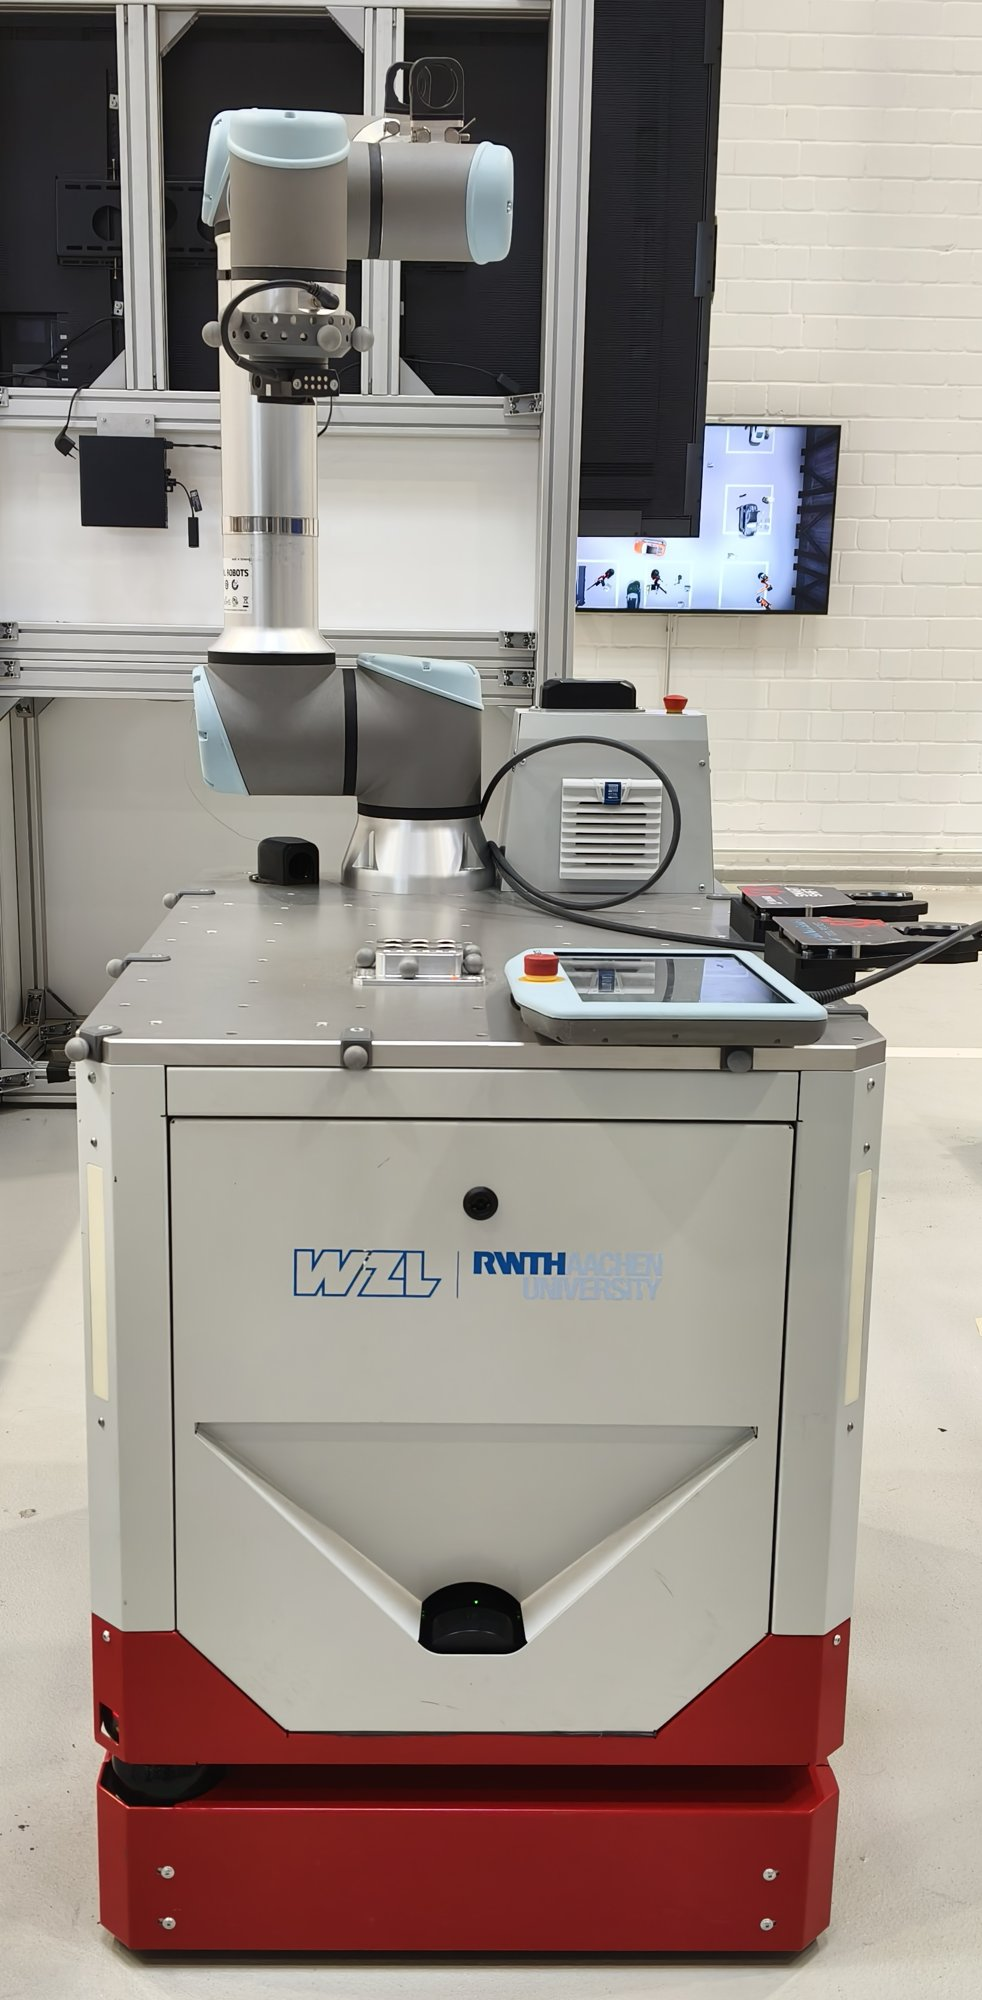
\includegraphics[width=\textwidth]{hero_view_front.jpg}
    \caption{Front}
    \label{fig:hero-photo-front}
  \end{subfigure}
  \hfill
  \begin{subfigure}[t]{0.34\textwidth}
    \centering
    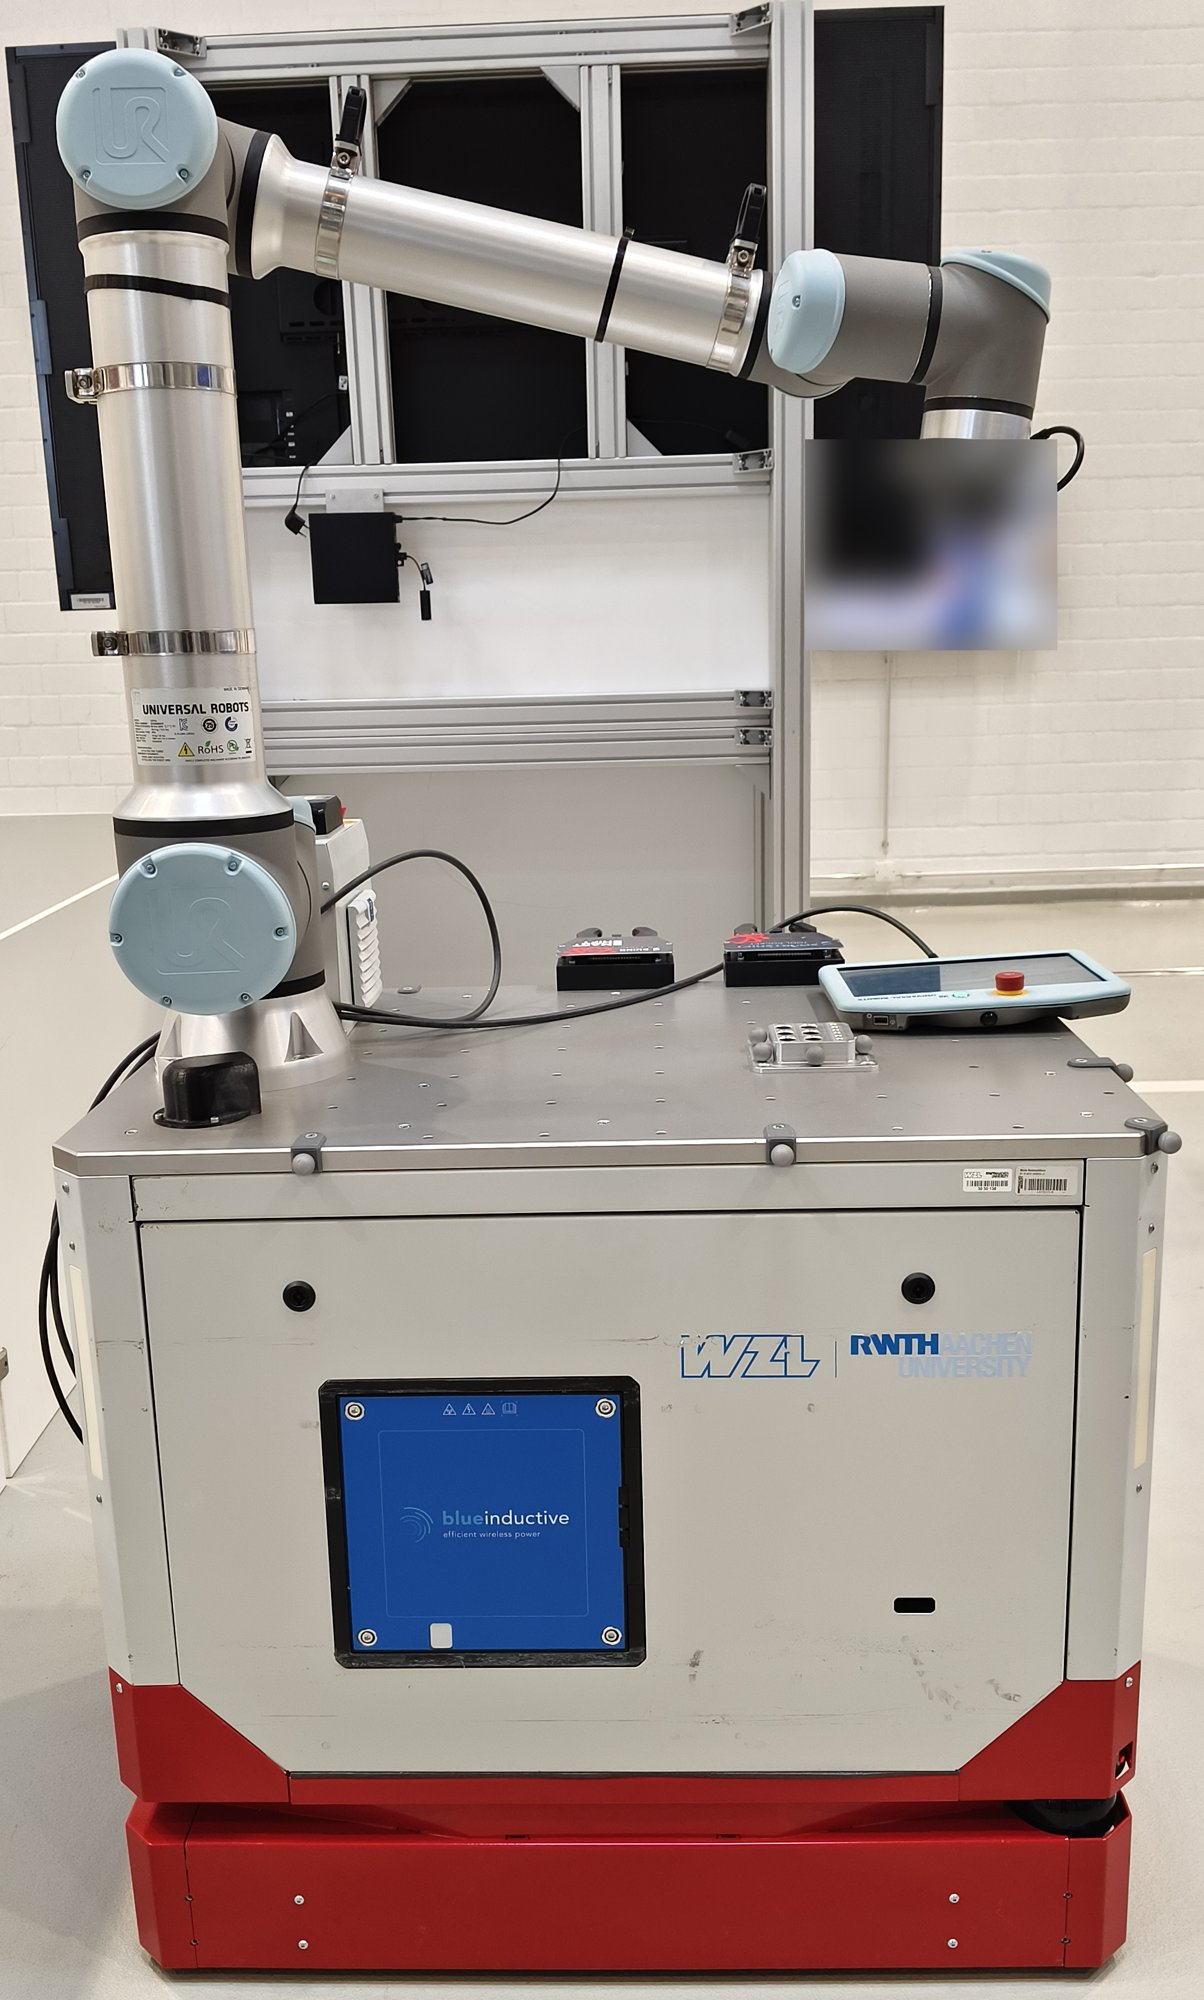
\includegraphics[width=\textwidth]{hero_view_side.jpg}
    \caption{Side}
    \label{fig:hero-photo-side}
  \end{subfigure}
  \hfill
  \begin{subfigure}[t]{0.27\textwidth}
    \centering
    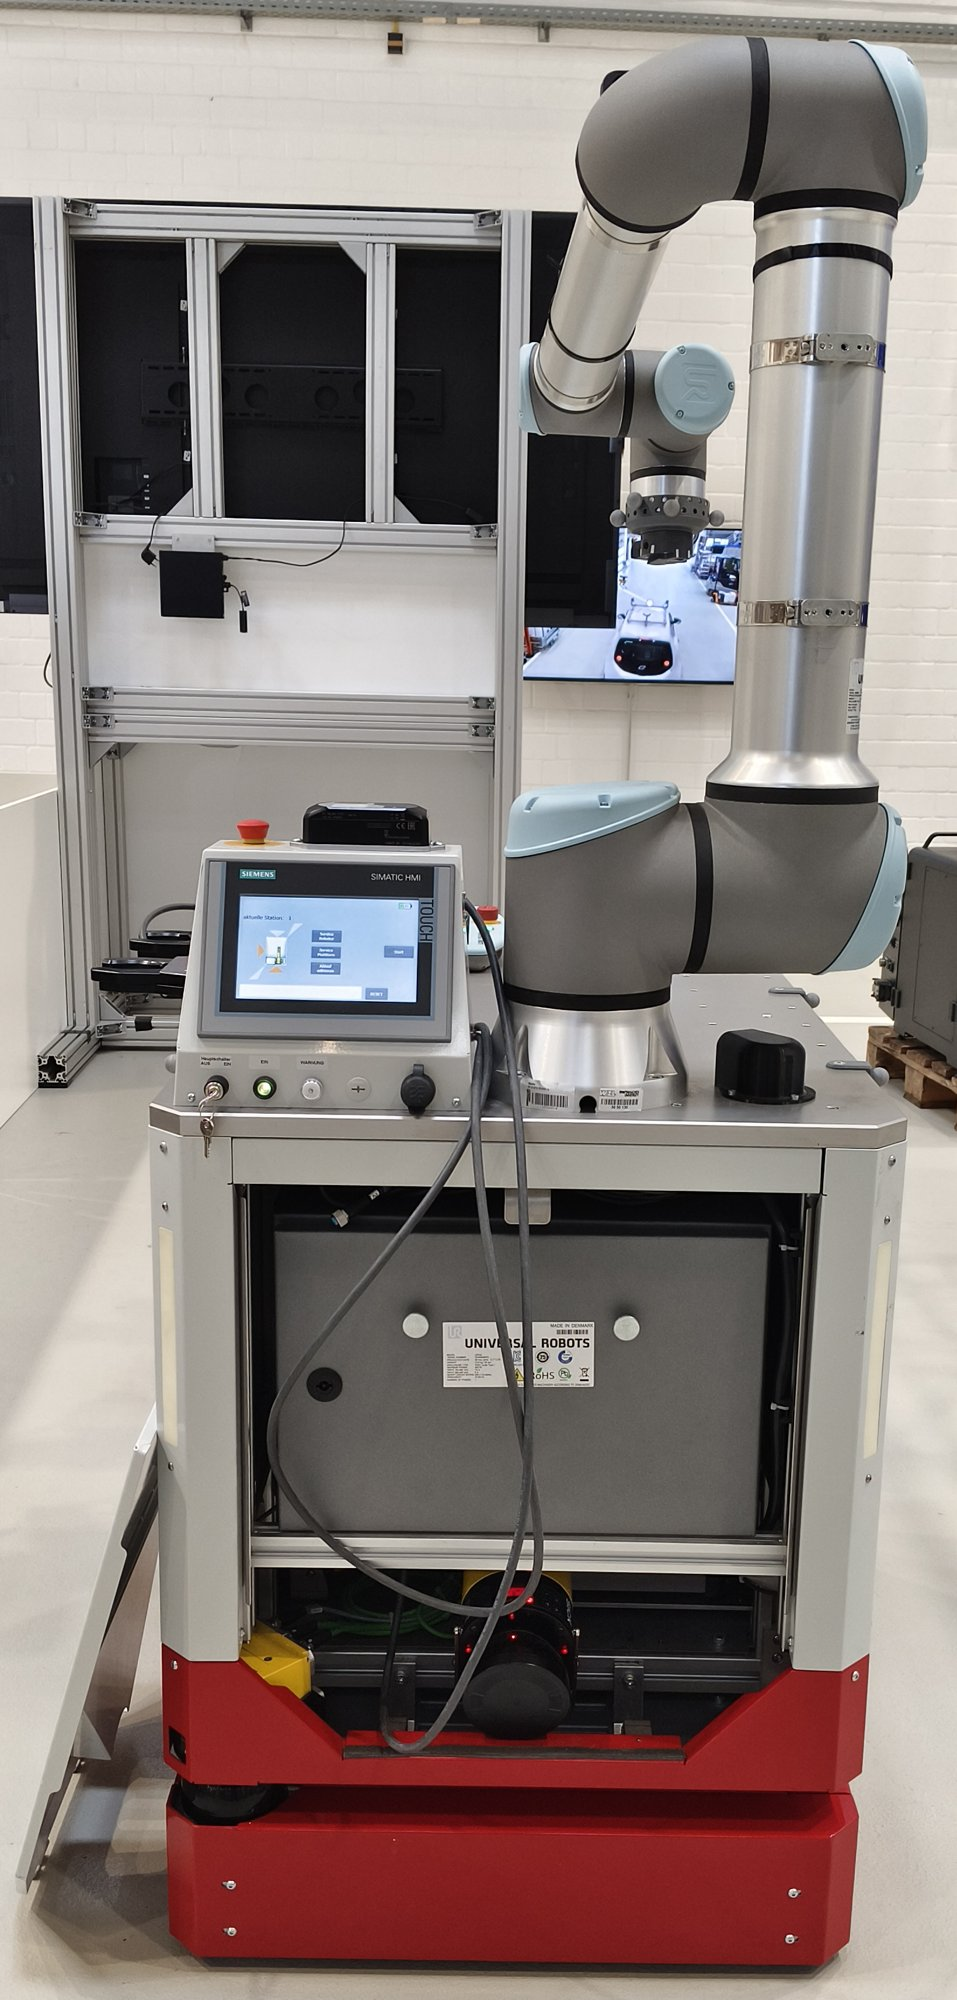
\includegraphics[width=\textwidth]{hero_view_back.jpg}
    \caption{Rear}
    \label{fig:hero-photo-rear}
  \end{subfigure}
  \caption{The \hero{} platform: UR10e arm on the \emph{freeMoVe} base
    with its red drive unit. The teach pendant lies on the top plate in
    (a) and (b). The operator panel next to the shoulder in (c) is the
    \texttt{hmi} link of the kinematic description; the UR control box
    sits inside the chassis below it.}
  \label{fig:hero-photo}
\end{figure}

Two properties of this combination shape the control problem. The first
is the drive geometry: the base pose has three planar degrees of freedom
but only two independent velocity inputs, and the base cannot translate
sideways~\cite{Lynch2017ModernRobotics}. A whole-body planner must
respect this non-holonomic restriction, otherwise it produces \ee{} paths
that the base cannot follow~\cite{Giftthaler2017Kinematic}. The second is
inertia. Moving a \qty{400}{\kilo\gram} platform is slow, and the safety
concept of the platform limits its speed independently of what a
controller may request, which is why the base velocities in
\cref{sec:wholebody-model} are capped an order of magnitude below the
arm's capability.

The kinematic tree is rooted at the frame \texttt{footprint}, which lies
on the ground plane midway between the drive wheels, with $x$ forward,
$y$ to the left and $z$ upwards. The controlled \ee{} frame is
\texttt{tool0}, the flange frame that coincides with the tool
orientation shown on the teach pendant; the arm's own
\texttt{base\_link} is not used, because its axes are rotated with
respect to the pendant convention and would invite sign errors when
comparing commanded and measured poses.

\Cref{fig:hero-frames} shows the tree, the frames it defines and the
state components attached to them.

\begin{figure}[htbp]
  \centering
  \begin{tikzpicture}[
      font=\footnotesize,
      box/.style={draw, rounded corners=1pt, align=center,
                  inner sep=3pt, minimum height=6.5mm, minimum width=23mm},
      passive/.style={box, fill=gray!12},
      ctrl/.style={box, draw=RWTHOrange100, thick},
      lbl/.style={font=\scriptsize, align=left},
      jt/.style={font=\scriptsize, align=center, inner sep=1.5pt},
      flow/.style={-{Latex[length=1.8mm]}, thick},
      note/.style={-{Latex[length=1.4mm]}, gray},
    ]
    % --- trunk ------------------------------------------------------
    \node[box]  (fp) at (0,0)     {\texttt{footprint}};
    \node[box]  (ch) at (0,-1.5)  {\texttt{chassis}};
    \node[box]  (mt) at (0,-3.4)  {\texttt{ur\_mount}};
    \node[box]  (bl) at (0,-4.7)  {\texttt{base\_link}};
    \node[box, minimum width=50mm] (ar) at (0,-6.2)
      {\texttt{shoulder\_link} $\to \cdots \to$ \texttt{wrist\_3\_link}};
    \node[ctrl] (t0) at (0,-7.7)  {\texttt{tool0}};

    % --- passive branches, all children of chassis -------------------
    \node[passive] (wh) at (4.9,-0.6) {\texttt{wheel\_left}\\\texttt{wheel\_right}};
    \node[passive] (cs) at (4.9,-2.0) {$4 \times$ caster};
    \node[passive] (hm) at (4.9,-3.1) {\texttt{hmi}};

    % --- trunk edges ------------------------------------------------
    \draw[flow] (fp) -- (ch) node[jt, midway, right=1mm] {fixed, identity};
    \draw[flow] (ch) -- (mt);
    \draw[flow] (mt) -- (bl) node[jt, midway, right=1mm] {fixed};
    \draw[flow] (bl) -- (ar) node[jt, midway, right=1mm] {6 revolute joints};
    \draw[flow] (ar) -- (t0) node[jt, midway, right=1mm] {fixed};

    % --- branch edges -----------------------------------------------
    \draw[flow] (ch.east) -- (wh.west) node[jt, pos=0.55, above, sloped] {continuous};
    \draw[flow] (ch.east) -- (cs.west);
    \draw[flow] (ch.east) -- (hm.west);

    % --- left-hand annotations --------------------------------------
    \node[lbl, anchor=east, text width=31mm] (npose) at (-2.2,0)
      {$(p_x, p_y, \psi)$: base pose\\in the inertial frame};
    \draw[note] (npose.east) -- (fp.west);

    \node[jt, anchor=east, align=right] at (-0.5,-2.45)
      {fixed,\\$(-0.355,\; -0.050,\; 0.830)\,\si{\meter}$,\\$R_z(\ang{-90})$};

    \node[lbl, anchor=east] (narm) at (-3.2,-6.2) {$\qarm \in \mathbb{R}^{6}$};
    \draw[note] (narm.east) -- (ar.west);

    % --- right-hand annotations -------------------------------------
    \node[lbl, anchor=west, text width=31mm] (nwh) at (6.3,-0.6)
      {declared \emph{fixed} in the\\Pinocchio model};
    \draw[note] (nwh.west) -- (wh.east);

    \node[lbl, anchor=west, text width=40mm] (nt0) at (2.0,-7.7)
      {controlled \ee{} frame;\\\texttt{base\_link} is not used\\as reference};
    \draw[note] (nt0.west) -- (t0.east);

    % --- footprint axes ---------------------------------------------
    \begin{scope}[shift={(-1.95,1.05)}]
      \draw[-{Latex[length=1.4mm]}] (0,0) -- (0.75,0) node[right, font=\scriptsize] {$x$};
      \draw[-{Latex[length=1.4mm]}] (0,0) -- (0,0.75) node[above, font=\scriptsize] {$z$};
      \draw[-{Latex[length=1.4mm]}] (0,0) -- (-0.45,-0.45)
        node[below left, font=\scriptsize, inner sep=1pt] {$y$};
    \end{scope}
  \end{tikzpicture}
  \caption[Kinematic tree and frame convention of \hero{}]{%
    Kinematic tree of \hero{} as the Pinocchio model sees it, with the
    transforms read from the platform description. The frame
    \texttt{footprint} lies on the ground plane midway between the drive
    wheels, at a track of \qty{0.548}{\meter} and a wheel radius of
    \qty{0.08}{\meter}. Shaded links carry no optimised degree of
    freedom: the two wheel joints are declared fixed, because the wheels
    are not part of the chain from base to \ee{}, and the casters and the
    operator panel are fixed in the description itself. The nine state
    components of \cref{eq:state-input} are attached to
    \texttt{footprint} and to the six revolute arm joints.}
  \label{fig:hero-frames}
\end{figure}

\Cref{fig:hero-frames} is a reduction. The transform tree that the
running system publishes has 51 frames and is shown in full in
\cref{fig:tf-tree}. Ten of its 50 transforms change over time: the base
pose, the six arm joints, the two wheel joints, and the pose of the
\ee{} target, which the \ocs{} visualisation adds for display. All
other frames are attachments, sensors and tool frames that are rigidly
fixed to one of the frames on the trunk.

\begin{figure}[htbp]
  \centering
  \begin{tikzpicture}[
      font=\scriptsize,
      fr/.style={draw, rounded corners=1pt, font=\scriptsize\ttfamily,
                 inner sep=2pt, minimum height=5mm, minimum width=31mm},
      side/.style={draw=gray, rounded corners=1pt, fill=gray!10,
                   font=\scriptsize\ttfamily\linespread{1}\selectfont,
                   align=left, inner sep=2.5pt, anchor=west},
      wide/.style={side, text width=76mm},
      sidemov/.style={side, draw=RWTHBlau100, fill=white},
      mov/.style={-{Latex[length=1.8mm]}, very thick, RWTHBlau100},
      fix/.style={-{Latex[length=1.6mm]}, thin},
      att/.style={gray},
      lbl/.style={font=\scriptsize\linespread{1}\selectfont, align=right},
      note/.style={-{Latex[length=1.4mm]}, gray},
    ]
    % --- trunk ------------------------------------------------------
    \node[fr] (world) at (0, 0)      {world};
    \node[fr] (fp)    at (0, -0.95)  {footprint};
    \node[fr] (ch)    at (0, -2.25)  {chassis};
    \node[fr] (mt)    at (0, -3.55)  {ur\_mount};
    \node[fr] (bl)    at (0, -4.5)   {base\_link};
    \node[fr] (bi)    at (0, -5.45)  {base\_link\_inertia};
    \node[fr] (sh)    at (0, -6.4)   {shoulder\_link};
    \node[fr] (ua)    at (0, -7.35)  {upper\_arm\_link};
    \node[fr] (fa)    at (0, -8.45)  {forearm\_link};
    \node[fr] (w1)    at (0, -9.5)   {wrist\_1\_link};
    \node[fr] (w2)    at (0, -10.4)  {wrist\_2\_link};
    \node[fr] (w3)    at (0, -11.3)  {wrist\_3\_link};
    \node[fr] (fl)    at (0, -12.2)  {flange};
    \node[fr] (t0)    at (0, -13.2)  {tool0};

    \draw[mov] (world) -- (fp);
    \draw[fix] (fp) -- (ch);
    \draw[fix] (ch) -- (mt);
    \draw[fix] (mt) -- (bl);
    \draw[fix] (bl) -- (bi);
    \draw[mov] (bi) -- (sh);
    \draw[mov] (sh) -- (ua);
    \draw[mov] (ua) -- (fa);
    \draw[mov] (fa) -- (w1);
    \draw[mov] (w1) -- (w2);
    \draw[mov] (w2) -- (w3);
    \draw[fix] (w3) -- (fl);
    \draw[fix] (fl) -- (t0);

    % --- frames that move but are not on the trunk -------------------
    \node[sidemov] (cmd) at (2.3, 0) {command};
    \draw[mov] (world.east) -- (cmd.west);
    \node[lbl, anchor=west, align=left] at (cmd.east)
      {\ee{} target, for display};
    \node[sidemov] (wh) at (2.3, -1.6) {wheel\_left, wheel\_right};
    \draw[mov] (ch.east) -- (wh.west);

    % --- frames rigidly attached to a trunk frame --------------------
    \node[wide] (chs) at (2.3, -2.95)
      {hmi\\
       caster\_front\_left, caster\_front\_right,
       caster\_rear\_left, caster\_rear\_right\\
       laser\_scanner\_front, laser\_scanner\_front\_right,
       laser\_scanner\_left, laser\_scanner\_rear,
       laser\_scanner\_rear\_left};
    \draw[att] (ch.east) -- (chs.west);
    \node[wide] (bls) at (2.3, -4.5)
      {base $\to$ \{platform\_markers, smartshift\_tool\_pocket\_A,
       smartshift\_tool\_pocket\_B\}};
    \draw[att] (bl.east) -- (bls.west);
    \node[side] (shs) at (2.3, -6.4) {ring1};
    \draw[att] (sh.east) -- (shs.west);
    \node[wide] (uas) at (2.3, -7.35)
      {ring2, ring2b, tube\_holder\_bottom\_1 $\to$ tmac\_box,
       tube\_holder\_bottom\_2};
    \draw[att] (ua.east) -- (uas.west);
    \node[wide] (fas) at (2.3, -8.45)
      {ring3, tube\_holder\_bottom\_3 $\to$ tube\_holder\_top\_3,
       tube\_holder\_bottom\_4 $\to$ tube\_holder\_top\_4};
    \draw[att] (fa.east) -- (fas.west);
    \node[side] (w1s) at (2.3, -9.5) {ring4};
    \draw[att] (w1.east) -- (w1s.west);
    \node[side] (w2s) at (2.3, -10.4) {ring5};
    \draw[att] (w2.east) -- (w2s.west);
    \node[side] (w3s) at (2.3, -11.3) {ft\_frame};
    \draw[att] (w3.east) -- (w3s.west);
    \node[wide] (t0s) at (2.3, -13.2)
      {ring6 $\to$ \{tool\_peg, tool\_tmac, smartshift\_robot\_adapter
       $\to$ smartshift\_tool\_adapter $\to$ tool\_smartshift\_mft\}};
    \draw[att] (t0.east) -- (t0s.west);

    % --- left-hand annotations --------------------------------------
    \node[lbl, anchor=west] at (0.2, -0.475)
      {base pose $(p_x, p_y, \psi)$};
    \node[lbl, anchor=east] (nfp) at (-2.3, -0.95)
      {model base frame};
    \draw[note] (nfp.east) -- (fp.west);
    \draw[RWTHBlau100, thick] (-1.85, -5.925) -- (-2.05, -5.925)
      -- (-2.05, -10.85) -- (-1.85, -10.85);
    \node[lbl, anchor=east] at (-2.2, -8.39)
      {six arm joints\\$\qarm \in \mathbb{R}^{6}$};
    \node[lbl, anchor=east] (nt0) at (-2.3, -13.2) {\ee{} frame};
    \draw[note] (nt0.east) -- (t0.west);

    % --- legend -----------------------------------------------------
    \draw[mov] (-3.9, -14.3) -- (-3.1, -14.3);
    \node[lbl, anchor=west] at (-3.0, -14.3) {changes over time};
    \draw[fix] (0.2, -14.3) -- (1.0, -14.3);
    \node[lbl, anchor=west] at (1.1, -14.3) {static};
    \node[side, minimum width=7mm, minimum height=3.2mm] at (3.0, -14.3) {};
    \node[lbl, anchor=west, align=left] at (3.8, -14.3)
      {frames fixed to the trunk frame on their left};
  \end{tikzpicture}
  \caption[Complete transform tree of \hero{}]{%
    Complete transform tree of \hero{}, redrawn from a
    \texttt{view\_frames} recording taken while the \ocs{} visualisation
    was running. The trunk runs from \texttt{world} to the \ee{} frame
    \texttt{tool0}. Thick blue arrows are the ten transforms that change
    over time; every other transform is static. A grey box lists the
    frames attached to the trunk frame on its left, and an arrow inside a
    box leads to a further child. The operator panel \texttt{hmi}, the
    tube holders and the marker rings \texttt{ring2} to \texttt{ring6}
    reappear among the bodies of the self-collision model in
    \cref{sec:wholebody-model}.}
  \label{fig:tf-tree}
\end{figure}

Beyond the drives, the platform carries five SICK safety laser scanners,
two safety controllers, wheel brakes, and an operator panel. None of
these enters the \mpc{} loop. The controller described here consumes
exactly two measurements, wheel odometry and arm joint positions, and
relies on the platform's own safety layer for protective stops. Obstacle
avoidance with respect to the environment is consequently not part of
the optimisation; only self-collision between the arm and the platform
is (\cref{sec:wholebody-model}).

Computation is split over two machines on the robot's own
\texttt{192.168.12.0/24} subnet. An industrial PC (IPC) inside the
platform hosts the ROS~2 Jazzy control stack in a container and reaches
the arm controller over the same subnet; an external PC joins
the subnet either by cable or through the platform's wireless access
point~\cite{ROS2,Macenski2022ROS2}. Which software runs where is the
subject of the next section.

% ---------------------------------------------------------------------
\section{Distributed System Architecture for Real-Time \mpc{}}
\label{sec:distributed-arch}

Solving the optimal-control problem is the most expensive part of the
loop relative to the remaining nodes on the IPC, and the IPC is the
smaller of the two machines available. It carries an Intel Core
i5-6300U with two cores and four threads and \qty{7.7}{\giga\byte} of
memory, runs a kernel without real-time patches, and keeps the CPU
frequency governor at \texttt{powersave}; the external PC carries an
AMD Ryzen~7 7840HS with eight cores and sixteen threads. The solver
alone is configured for eight threads (\cref{tab:mpc-config}), twice
what the IPC offers before the control chain takes its share, so
running it on board would have forced a shorter horizon or a coarser
model.

The MPC--MRT split of \ocs{} (\cref{sec:sota-ocs2}) removes that
constraint: the optimiser and the client that evaluates its policy are
separate processes that exchange messages, so they may live on
different machines~\cite{ocs2Toolbox}.

The deployment used here puts them on either side of the machine
boundary. The external PC runs the \mpc{} node, the target-generating
node and the visualisation, while the IPC runs the low-level control
chain and the MRT bridge. The fast path---measure, evaluate the policy,
actuate---is then entirely local to the IPC, and only three \ocs{}
streams cross the machine boundary. \Cref{tab:topology-streams} lists
what runs where and what the network carries.

\begin{table}[htbp]
  \centering
  \caption[Process placement and traffic across the machine boundary]{%
    Process placement and the traffic that crosses the external
    PC--IPC boundary. Keeping the MRT bridge on the IPC is what leaves
    the actuation path machine-local.}
  \label{tab:topology-streams}
  \begin{tabularx}{\linewidth}{@{}lX@{}}
    \toprule
    External PC
      & \mpc{} node, target node, RViz \\
    IPC
      & control chain, MRT bridge \\
    \addlinespace
    Crossing the network
      & \texttt{\_mpc\_observation} (IPC\,$\rightarrow$\,external PC,
        \qty{50}{\hz}), \texttt{\_mpc\_policy}
        (external PC\,$\rightarrow$\,IPC), \texttt{\_mpc\_reset} service
        at start-up \\
    \addlinespace
    Effect of a link outage
      & the bridge keeps evaluating the last policy locally until its
        validity window expires, then holds \\
    Clock synchronisation
      & not required \\
    \bottomrule
  \end{tabularx}
\end{table}

The last of those rows follows from where wall-clock times are compared.
\ocs{} timestamps observations and policies on a relative time axis
whose origin the bridge fixes at the first accepted measurement, so the
\mpc{}--MRT exchange itself is insensitive to an offset between the two
machine clocks. The bridge does compare wall-clock times in one place,
its staleness check on incoming measurements, and there the two operands
share the IPC clock: the bridge runs on the IPC, and odometry and joint
states are published by the control chain on the same machine. An offset
to the external PC therefore never enters the \qty{0.2}{\second}
staleness threshold, and a time service such as Chrony is not needed to
keep the loop running~\cite{Chrony}. Chrony does run on the IPC, with
the external PC as its reference; at the time of writing it reported an
offset of \qty{-0.7}{\milli\second} at an RMS of
\qty{1.5}{\milli\second}. That keeps logs recorded on the two machines
comparable, but the control loop does not depend on it.

The deployment runs with the Zenoh middleware implementation rather than
the default DDS transport of ROS~2. The switch was made during
bring-up, after DDS discovery over the platform's wireless link had
repeatedly failed to establish the \ocs{} streams; no side-by-side
comparison of the two middlewares was recorded, so this is a deployment
decision and not a measured result~\cite{zenoh,Macenski2022ROS2}.
Zenoh requires a router process on each machine, with one router
configured to connect to the other; the external PC router is pointed at
the IPC router. \Cref{fig:architecture} shows the resulting node and
topic layout.

\begin{figure}[htbp]
  \centering
  \begin{tikzpicture}[
      font=\footnotesize,
      box/.style={draw, rounded corners=1pt, align=center,
                  inner sep=4pt, minimum height=9mm},
      machine/.style={draw, dashed, rounded corners=2pt, inner sep=7pt},
      flow/.style={-{Latex[length=2mm]}, thick},
      lbl/.style={font=\scriptsize, align=center},
    ]
    % --- PC ------------------------------------------------
    \node[box, minimum width=30mm] (mpc)    at (0,0)
      {\mpc{} node\\(SLQ solver)};
    \node[box, minimum width=32mm] (target) at (-4.9,0)
      {target node\\(\ee{} reference)};
    \node[machine, fit=(mpc)(target),
          label={[lbl]above:external PC}] (host) {};

    % --- IPC --------------------------------------------------------
    \node[box, minimum width=34mm] (mrt)  at (0,-3.8)
      {MRT bridge\\(policy evaluation)};
    \node[box, minimum width=40mm] (ctrl) at (0,-6.1)
      {\texttt{ros2\_control}\\twist\_mux, diff.\ drive, JTC};
    \node[box, minimum width=30mm] (rsp)  at (-4.9,-6.1)
      {\texttt{robot\_state\_}\\\texttt{publisher}};
    \node[inner sep=0pt, minimum size=0pt] (pad) at (2.9,-4.95) {};
    \node[machine, fit=(mrt)(ctrl)(rsp)(pad),
          label={[lbl]below:On-board IPC}] (ipc) {};

    % --- robot ------------------------------------------------------
    \node[box, minimum width=30mm] (robot) at (0,-8.3)
      {wheels, UR10e};

    % --- cross-machine streams --------------------------------------
    \draw[flow] ([xshift=-7mm]mrt.north) -- ([xshift=-7mm]mpc.south)
      node[lbl, pos=0.35, left=1mm] {observation\\\qty{50}{\hz}};
    \draw[flow] ([xshift=7mm]mpc.south) -- ([xshift=7mm]mrt.north)
      node[lbl, pos=0.32, right=1mm] {policy};

    % --- local links ------------------------------------------------
    \draw[flow] (target) -- (mpc)
      node[lbl, midway, above] {reference};
    \draw[flow] ([xshift=-7mm]mrt.south) -- ([xshift=-7mm]ctrl.north)
      node[lbl, midway, left=1mm] {base twist,\\arm trajectory};
    \draw[flow] ([xshift=7mm]ctrl.north) -- ([xshift=7mm]mrt.south)
      node[lbl, midway, right=1mm] {odometry,\\joint states};
    \draw[flow, {Latex[length=2mm]}-{Latex[length=2mm]}]
      (ctrl.south) -- (robot.north);
    \draw[flow, dashed] (ctrl.west) -- (rsp.east)
      node[lbl, midway, above=0.5mm] {joint states};

    % --- network boundary -------------------------------------------
    \draw[dotted, thick] (-7.3,-1.9) -- (3.0,-1.9);
    \node[lbl, anchor=west] at (-7.3,-2.15) {Zenoh network boundary};
  \end{tikzpicture}
  \caption[Deployment of \ocs{} on \hero{}]{%
    Deployment of \ocs{} on \hero{}. The external PC solves the
    optimal-control problem; the IPC evaluates the resulting policy and
    actuates the robot, so the loop that runs at \qty{50}{\hz} is
    machine-local. The reset service and the visualisation on the
    external PC are omitted.}
  \label{fig:architecture}
\end{figure}

One consistency requirement is easy to violate and is stated here
explicitly. The \mpc{} node and the MRT bridge each build their own
Pinocchio model from a URDF file that is exported from the platform
description at launch time~\cite{Carpentier2019Pinocchio}. The two
exports must use the same end-effector variant and the same kinematic
calibration file, otherwise the solver optimises for one robot and the
bridge evaluates the policy on another. The visualisation, in contrast, takes its model from the
\texttt{robot\_state\_publisher} on the IPC, which is the single
authoritative source of \texttt{/tf} and \texttt{/robot\_description};
the external PC launch deliberately starts no second publisher. Because
\ocs{} hardcodes \texttt{world} as its inertial frame while the robot
tree is rooted at \texttt{odom}, an identity transform between the two
is published on the external PC. The base state fed to the solver is
wheel odometry, so \texttt{world} and \texttt{odom} coincide
numerically; the price is that the controller inherits the drift of the
odometry, and no external localisation corrects it.

Start-up follows a fixed order: the Zenoh routers first, then the
\mpc{} node on the external PC, then the IPC. The \mpc{} node advertises
the reset service that the bridge needs for its initial handshake, so
starting it first avoids a wait. The reverse order also converges,
because the bridge waits for the service rather than aborting
(\cref{sec:hw-interfaces}). On the first start after a model change,
\ocs{} generates and compiles the derivative code before the solver
runs, which adds a delay of roughly one minute; the compiled libraries
are then cached on disk.

% ---------------------------------------------------------------------
\section{Whole-Body Model and Parameterisation}
\label{sec:wholebody-model}

\ocs{} ships a mobile-manipulator model family, of which the
\emph{wheel-based} variant matches \hero{}: a non-holonomic planar base
carrying a serial arm~\cite{ocs2Toolbox}. The Pinocchio model is built
from the platform URDF with the two wheel joints declared fixed, since
the wheels are not part of the kinematic chain from base to \ee{} and
their rotation is irrelevant to the
task~\cite{Carpentier2019Pinocchio}. The base frame is \texttt{footprint}
and the \ee{} frame is \texttt{tool0}, as introduced in
\cref{sec:hero-platform}. The resulting state and input are

\begin{equation}
  \svec = \left( p_x,\; p_y,\; \psi,\; \qarm \right) \in \mathbb{R}^{9},
  \qquad
  \uvec = \left( v,\; \omega,\; \qarmdot \right) \in \mathbb{R}^{8},
  \label{eq:state-input}
\end{equation}

with $(p_x, p_y, \psi)$ the base pose in the inertial frame,
$\qarm \in \mathbb{R}^{6}$ the arm joint positions, $v$ and $\omega$ the
base forward and yaw rate, and $\qarmdot$ the arm joint velocities.
The system equation is the differential-drive kinematics augmented by
the arm joints~\cite{Lynch2017ModernRobotics},

\begin{equation}
  \dot{\svec} \;=\; f(\svec, \uvec) \;=\;
  \begin{pmatrix}
    v \cos\psi \\ v \sin\psi \\ \omega \\ \qarmdot
  \end{pmatrix} ,
  \label{eq:flowmap}
\end{equation}

which encodes the non-holonomic restriction of
\cref{sec:hero-platform}: no input produces motion along the base
$y$-axis. The model is kinematic, not dynamic. The control chain used
here issues only a twist to the drive controller and position setpoints,
at a fixed rate, to the joint-trajectory controller. No validated
inertial parameters exist for the loaded platform either. A dynamic
model would therefore add eight velocity states ($v$, $\omega$ and the
six arm joint rates) and an unverified mass matrix, while the commands
that reach the actuators would remain twists and joint positions. The
cost of this choice is that inertial effects appear to the solver only
through the velocity limits.

The objective combines an input cost with soft constraints. Over a
horizon $T$ starting at $t_0$,

\begin{equation}
  \begin{aligned}
    J = \int_{t_0}^{t_0+T} \Big[
        &\tfrac{1}{2}\, \uvec^{\mathsf{T}} R\, \uvec
      + \tfrac{1}{2}\, \mu_\mathrm{p} \lVert e_\mathrm{p}(\svec) \rVert^2
      + \tfrac{1}{2}\, \mu_\mathrm{o} \lVert e_\mathrm{o}(\svec) \rVert^2 \\
      &+ B_\mathrm{lim}(\svec, \uvec) + B_\mathrm{col}(\svec)
      \Big]\, \mathrm{d}t
      \;+\; \Phi\big(\svec(t_0+T)\big) ,
  \end{aligned}
  \label{eq:cost}
\end{equation}

where $e_\mathrm{p}$ is the \ee{} position error and $e_\mathrm{o}$ the
orientation error, both taken with respect to the reference pose
interpolated from the target trajectory at the current time, and $\Phi$
repeats the two \ee{} terms at the end of the horizon. The reference is
supplied online through the \ocs{} reference manager, either by an
interactive marker in RViz or by the waypoint node used in
\cref{ch:simulation,ch:hardware}. \ocs{} interpolates that reference
linearly and component-wise between successive knots, the quaternion
included, which is why the waypoint node commands one constant
orientation for the whole path (\cref{sec:sim-path}).
\Cref{fig:cost-structure} collects the terms and the quantities each of
them acts on.

\begin{figure}[htbp]
  \centering
  \begin{tikzpicture}[
      font=\footnotesize,
      term/.style={draw, rounded corners=1pt, align=center, inner sep=3.5pt,
                   minimum height=7.5mm, minimum width=30mm},
      tgt/.style={draw, rounded corners=1pt, align=center, inner sep=3.5pt,
                  minimum height=7.5mm, minimum width=36mm, fill=gray!10},
      ref/.style={draw, rounded corners=1pt, align=center, inner sep=3pt,
                  minimum height=6.5mm, minimum width=36mm,
                  draw=RWTHBlau100},
      flow/.style={-{Latex[length=1.8mm]}, thick},
      wk/.style={font=\scriptsize, align=left},
      lbl/.style={font=\scriptsize, align=center},
    ]
    % --- cost terms ---------------------------------------------------
    \node[term] (r)   at (0,0)    {$\tfrac{1}{2}\,\uvec^{\mathsf{T}} R\, \uvec$};
    \node[term] (ep)  at (0,-1.15) {$\tfrac{1}{2}\, \mu_\mathrm{p} \lVert e_\mathrm{p} \rVert^2$};
    \node[term] (eo)  at (0,-2.30) {$\tfrac{1}{2}\, \mu_\mathrm{o} \lVert e_\mathrm{o} \rVert^2$};
    \node[term] (bl)  at (0,-3.45) {$B_\mathrm{lim}(\svec, \uvec)$};
    \node[term] (bc)  at (0,-4.60) {$B_\mathrm{col}(\svec)$};
    \node[term] (phi) at (0,-5.75) {$\Phi\big(\svec(t_0+T)\big)$};

    % --- configured values --------------------------------------------
    \node[wk, anchor=east] at (-1.75,0)     {$R_\mathrm{base} = 0.085\, I_2$,\\$R_\mathrm{arm} = 0.04\, I_6$};
    \node[wk, anchor=east] at (-1.75,-1.15) {$\mu_\mathrm{p} = 10$};
    \node[wk, anchor=east] at (-1.75,-2.30) {$\mu_\mathrm{o} = 5$};
    \node[wk, anchor=east] at (-1.75,-3.45) {panel joint limits,\\velocity bounds on all\\eight inputs};
    \node[wk, anchor=east] at (-1.75,-4.60) {12 link pairs,\\margin \qty{0.11}{\meter}};
    \node[wk, anchor=east] at (-1.75,-5.75) {repeats $\mu_\mathrm{p}$, $\mu_\mathrm{o}$\\at the horizon end};

    % --- targets --------------------------------------------------------
    \node[tgt] (u) at (5.2,0)     {input $\uvec = (v, \omega, \qarmdot)$};
    \node[tgt] (e) at (5.2,-1.95) {\ee{} pose error against\\the reference pose};
    \node[tgt] (x) at (5.2,-4.30) {state $\svec$};

    % --- reference chain -------------------------------------------------
    \node[ref] (src) at (5.2,-6.5)
      {interactive marker or\\waypoint node};
    \node[ref] (int) at (5.2,-8.0)
      {component-wise linear\\interpolation, quaternion\\included};
    \draw[flow, RWTHBlau100] (src) -- (int);
    \draw[flow, RWTHBlau100] (int.east) -- ++(1.1,0) |- (e.east);

    % --- term to target ---------------------------------------------------
    \draw[flow] (r)   -- (u);
    \draw[flow] (ep.east)  -- (e.west);
    \draw[flow] (eo.east)  -- (e.west);
    \draw[flow] (bl.east)  -- (x.west);
    \draw[flow] (bl.east)  -- (u.west);
    \draw[flow] (bc.east)  -- (x.west);
    \draw[flow, dashed] (phi.east) -- (2.75,-5.75) |- ([yshift=-2.5mm]e.west);
  \end{tikzpicture}
  \caption[Structure of the \ocs{} objective on \hero{}]{%
    Terms of the objective in \cref{eq:cost}, the values configured for
    them in \cref{tab:mpc-config}, and the quantities each term acts on.
    The ratio between $R_\mathrm{base}$ and $R_\mathrm{arm}$ is what
    distributes a commanded \ee{} motion between base and arm. In blue,
    the path by which the reference reaches the two \ee{} terms: the
    reference manager interpolates between successive knots
    component-wise, the quaternion included, which is why the waypoint
    node commands one constant orientation for a whole path.}
  \label{fig:cost-structure}
\end{figure}

The input weight is diagonal and separates base from arm,
$R = \operatorname{diag}(R_\mathrm{base}, R_\mathrm{arm})$ with
$R_\mathrm{base} = 0.085 \cdot I_2$ and
$R_\mathrm{arm} = 0.04 \cdot I_6$. The ratio is the tuning knob that
distributes a commanded \ee{} motion between base and arm: base motion
is charged roughly twice as much as arm motion, which keeps the heavy
platform still for targets the arm can reach on its own and lets it
contribute once the arm approaches its reach limit. \Cref{ch:hardware}
returns to this ratio, because it also determines whether the base
starts moving early enough for paths that leave the arm's workspace.

Limits and self-collision enter as relaxed barrier penalties, the
\ocs{} treatment of an inequality
$h(\svec,\uvec) \ge 0$~\cite{Feller2017RelaxedBarrier,ocs2Toolbox}:

\begin{equation}
  B(h) =
  \begin{cases}
    -\mu \ln h, & h > \delta, \\[2pt]
    -\mu \ln \delta
      + \dfrac{\mu}{2}\left[ \left(\dfrac{h - 2\delta}{\delta}\right)^{2} - 1 \right],
      & h \le \delta .
  \end{cases}
  \label{eq:barrier}
\end{equation}

The barrier is logarithmic while the constraint is comfortably
satisfied and switches to a quadratic extension below the relaxation
width $\delta$, which keeps the cost and its derivatives finite when a
constraint is violated---necessary here, because measured states from
the real robot do occasionally violate a limit. \Cref{fig:barrier}
shows the penalty at the configured relaxation width.

\begin{figure}[htbp]
  \centering
  \begin{tikzpicture}
    \begin{axis}[
        width=0.88\linewidth, height=5.2cm,
        xlabel={constraint slack $h$ / \si{\milli\meter}},
        ylabel={$B(h)$},
        xmin=-3, xmax=20, ymin=0, ymax=0.2,
        scaled y ticks=false,
        yticklabel style={/pgf/number format/fixed,
                          /pgf/number format/precision=2},
        legend pos=north east,
      ]
      \addplot[RWTHOrange100, thick, domain=-3:1, samples=90]
        {-0.01*ln(0.001) + 0.005*((x-2)^2 - 1)};
      \addplot[RWTHBlau100, thick, domain=1:20, samples=200]
        {-0.01*ln(x/1000)};
      \addplot[black, dashed, forget plot] coordinates {(1,0) (1,0.2)};
      \legend{quadratic extension, $-\mu \ln h$}
      \node[anchor=south west, font=\scriptsize] at (axis cs:1.3,0.155)
        {$\delta = \qty{1}{\milli\meter}$};
    \end{axis}
  \end{tikzpicture}
  \caption[Relaxed barrier penalty at the configured relaxation width]{%
    Relaxed barrier penalty of \cref{eq:barrier} at the values configured
    for the self-collision term, $\mu = \num{e-2}$ and
    $\delta = \qty{1}{\milli\meter}$. The slack $h$ is the amount by
    which a constraint is satisfied, so $h = 0$ is the constraint
    boundary and $h < 0$ a violation. Left of $\delta$ the logarithm is
    replaced by its quadratic extension, which keeps the penalty and its
    derivatives finite for the violated states that the real robot
    occasionally reports. For self-collision the slack is the distance of
    a link pair minus the \qty{0.11}{\meter} margin, so the quadratic
    extension acts only on a pair that is closer than
    $\qty{0.11}{\meter} + \delta$.}
  \label{fig:barrier}
\end{figure}

Three groups of
constraints use this penalty: arm joint position limits, velocity limits
on all eight inputs, and a minimum distance between selected pairs of
links. The position limits are overridden in the task file instead of
being read from the URDF, which bounds every UR10e joint at
\ang{\pm 360}. Those bounds are far wider than the joint limits
configured in the arm's own safety panel, so a plan that satisfies the
URDF can still drive the arm into a safety limit and provoke a
protective stop that \ocs{} never sees. The task file therefore copies
the Normal-mode panel limits of the installation used in this work
(\cref{fig:pendant-limits}): \ang{-183} to \ang{3} for the base and
shoulder joints, \ang{\pm 153} for the elbow, \ang{-228} to \ang{48}
for wrist~1, \ang{\pm 138} for wrist~2 and \ang{\pm 183} for wrist~3.
The velocity bounds are \qty{\pm 0.1}{\meter\per\second} and
\qty{\pm 0.1}{\radian\per\second} for the base and
\qty{\pm 0.3}{\radian\per\second} per arm joint, matching the caps that
the bridge enforces downstream (\cref{sec:hw-interfaces}).

\begin{figure}[htbp]
  \centering
  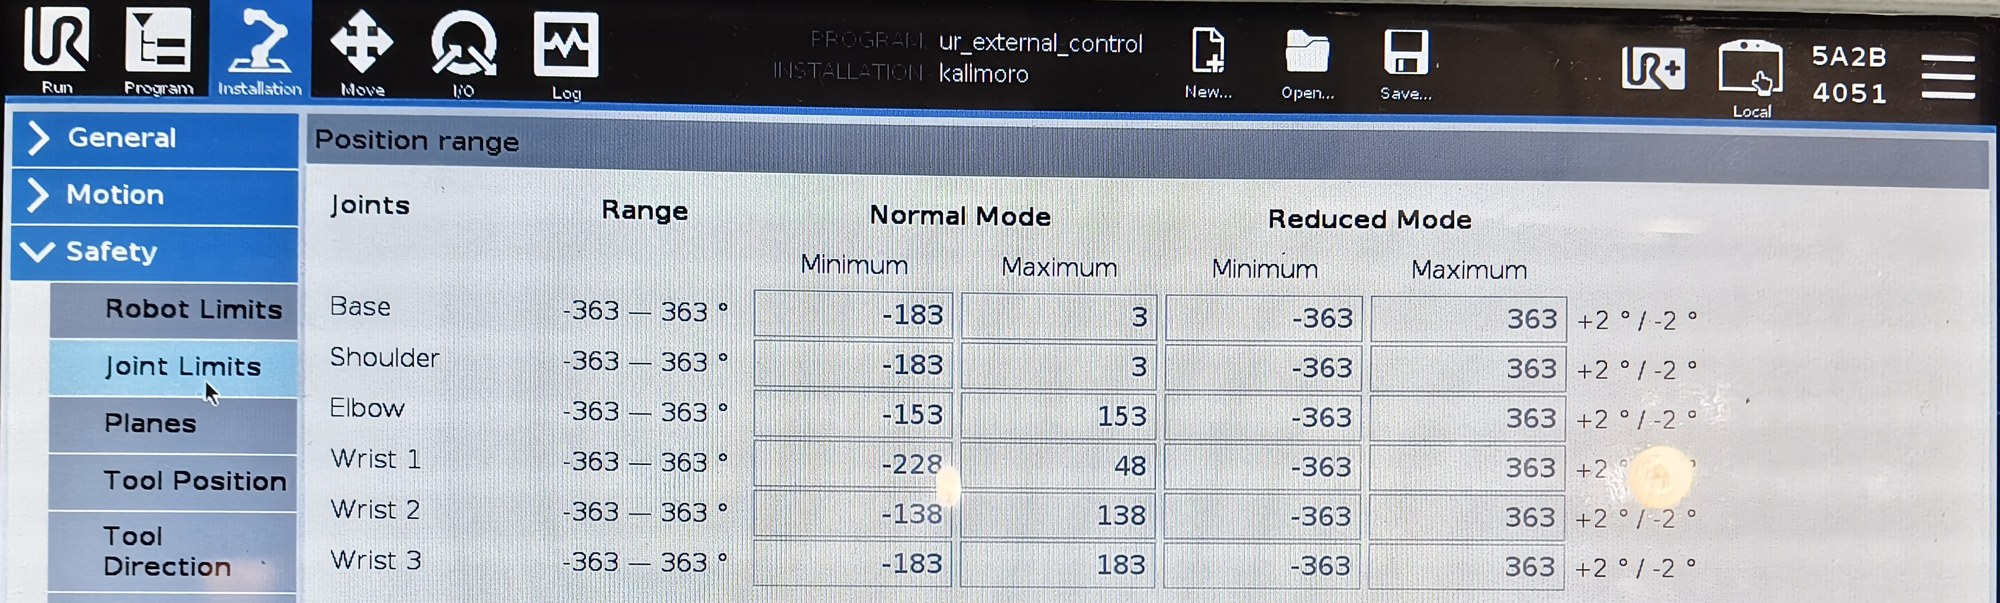
\includegraphics[width=\textwidth]{ur_pendant_joint_limits.jpg}
  \caption{Joint-limit page of the UR10e safety configuration on the
    teach pendant, installation \texttt{kalimoro}. The Normal-mode
    ranges equal the bounds in \texttt{task\_hardware.info}; the
    Reduced-mode ranges are not used in this work.}
  \label{fig:pendant-limits}
\end{figure}

Self-collision is singled out here because its evaluation cost scales
with the number of geometry pairs, and it was therefore the first term
addressed when solve time had to be reduced. Every pair costs a distance
query and its derivative with respect to the state at each node of the
time grid on which the solver linearises the
problem~\cite{Carpentier2019Pinocchio}. That grid comes from the
rollout and not from the \qty{2}{\milli\second} step at which the
backward pass integrates the Riccati equation; since the rollout
integrates adaptively, the number of nodes follows the solution rather
than the horizon~\cite{ocs2Toolbox}. It can be counted from the
recordings, because a published policy carries the solver's own grid
without resampling: over the 713 policies of the hardware lap of
\cref{ch:hardware}, one solve spans a median of ten nodes across the
\qty{1.24}{\second} it publishes, with a quartile range of nine to ten,
and the first interval equals the requested
\qty{10}{\milli\second} rollout step of \cref{tab:mpc-config} in every
one of them. Cutting the pair set from 32 to 12 therefore removes about
two hundred distance queries, and as many derivative evaluations, from
each solve. The constraint value of a pair is its distance minus the
minimum distance~\cite{ocs2Toolbox}.

Two platform bodies are within reach of the arm. The chassis top is the
mounting plane of the arm, and the shoulder axis lies only about
\qty{0.18}{\meter} above it; the operator panel (\texttt{hmi}), a box of
\qty{0.21}{\meter} $\times$ \qty{0.30}{\meter} $\times$
\qty{0.25}{\meter}, starts \qty{0.075}{\meter} beside the shoulder axis
and covers the height of the shoulder. On the arm side, the five moving
links from \texttt{upper\_arm\_link} to \texttt{wrist\_3\_link} carry
attachments: six marker rings of the motion capture system, which
protrude at most about \qty{1}{\centi\meter} from the link surface, and
six tube holders, which protrude about
\qtyrange{3}{6}{\centi\meter} (\cref{fig:collision-photos}). Pairing both platform bodies with these links and
attachments gave the original set of 32 pairs. Pairs whose distance does
not change with the arm configuration, such as the shoulder link against
the chassis, were never part of it.

\begin{figure}[htbp]
  \centering
  \begin{subfigure}[t]{0.40\textwidth}
    \centering
    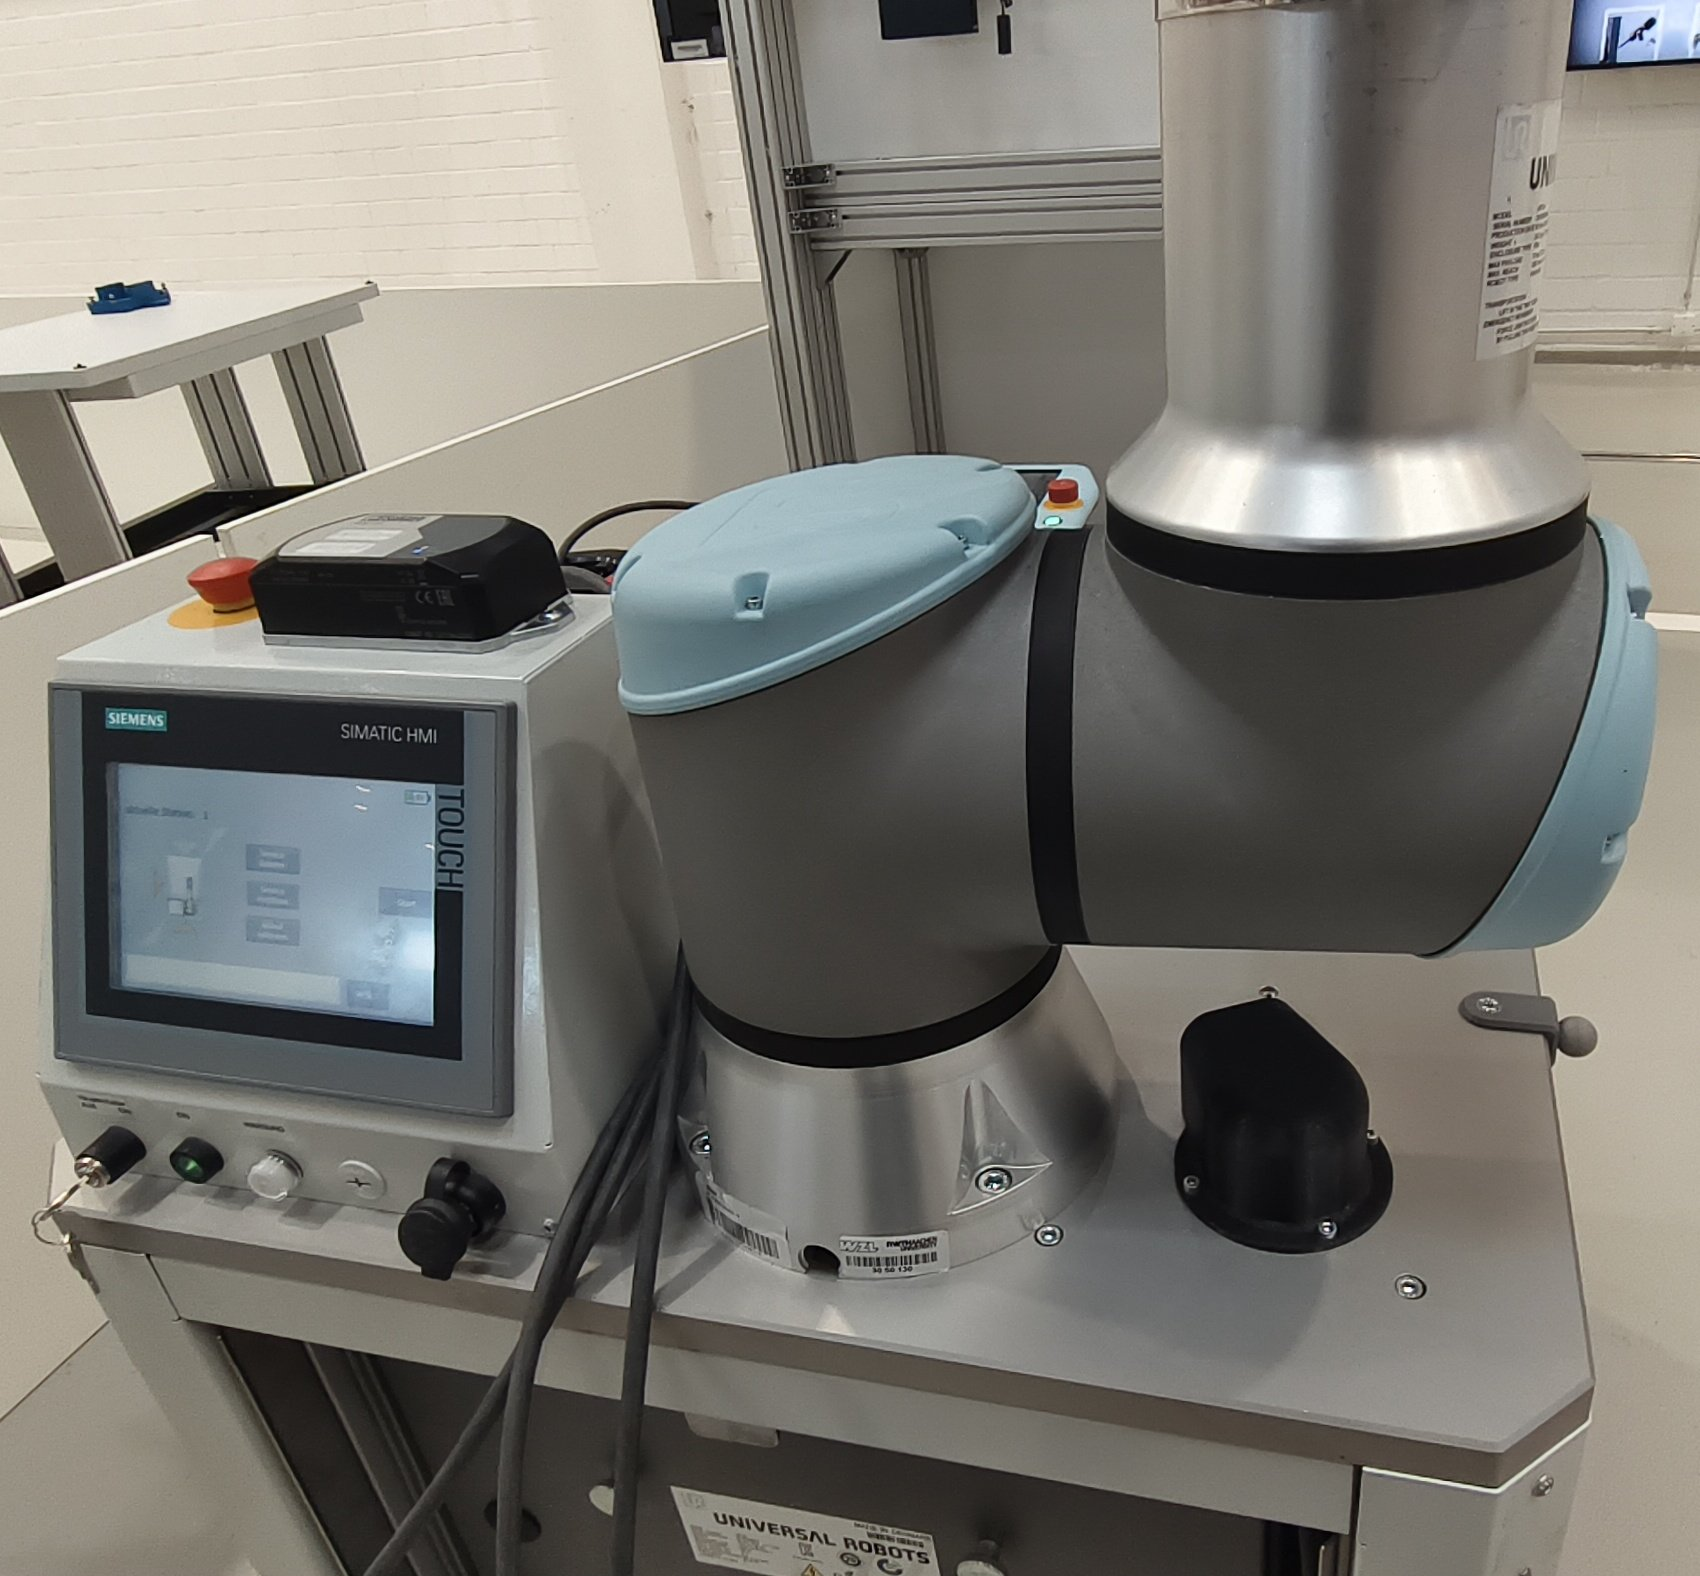
\includegraphics[height=5cm]{hero_arm_mount.jpg}
    \caption{Arm base on the chassis top, next to the operator panel
      (\texttt{hmi}).}
    \label{fig:collision-photo-mount}
  \end{subfigure}
  \hfill
  \begin{subfigure}[t]{0.27\textwidth}
    \centering
    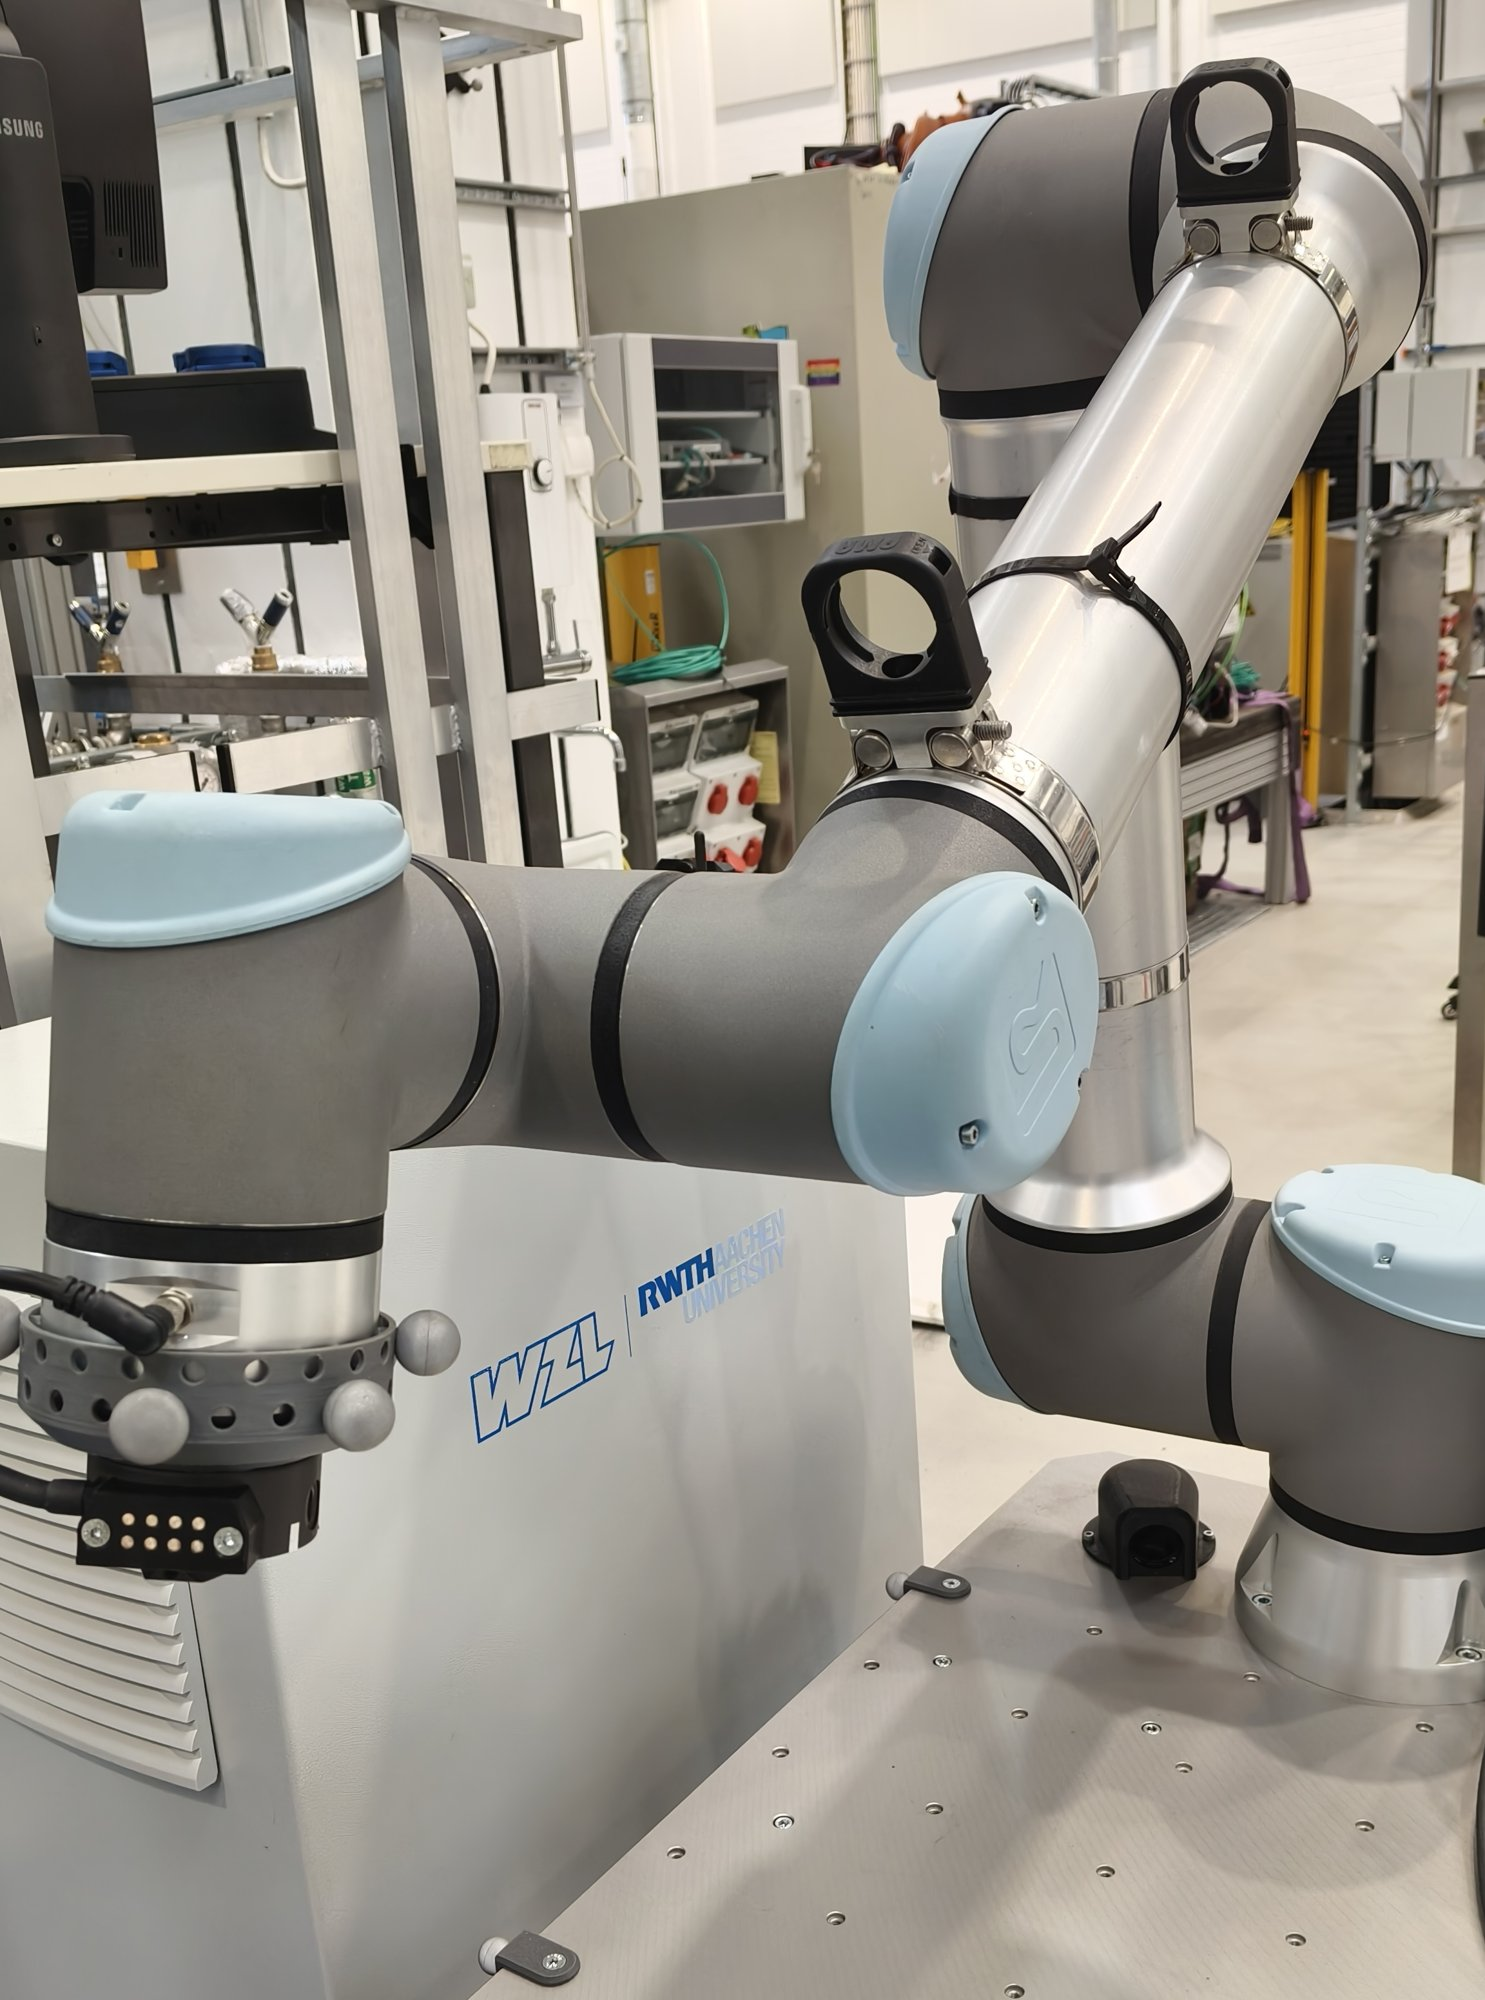
\includegraphics[height=5cm]{hero_tube_holders.jpg}
    \caption{Tube holders on the upper arm and the forearm.}
    \label{fig:collision-photo-tubes}
  \end{subfigure}
  \hfill
  \begin{subfigure}[t]{0.27\textwidth}
    \centering
    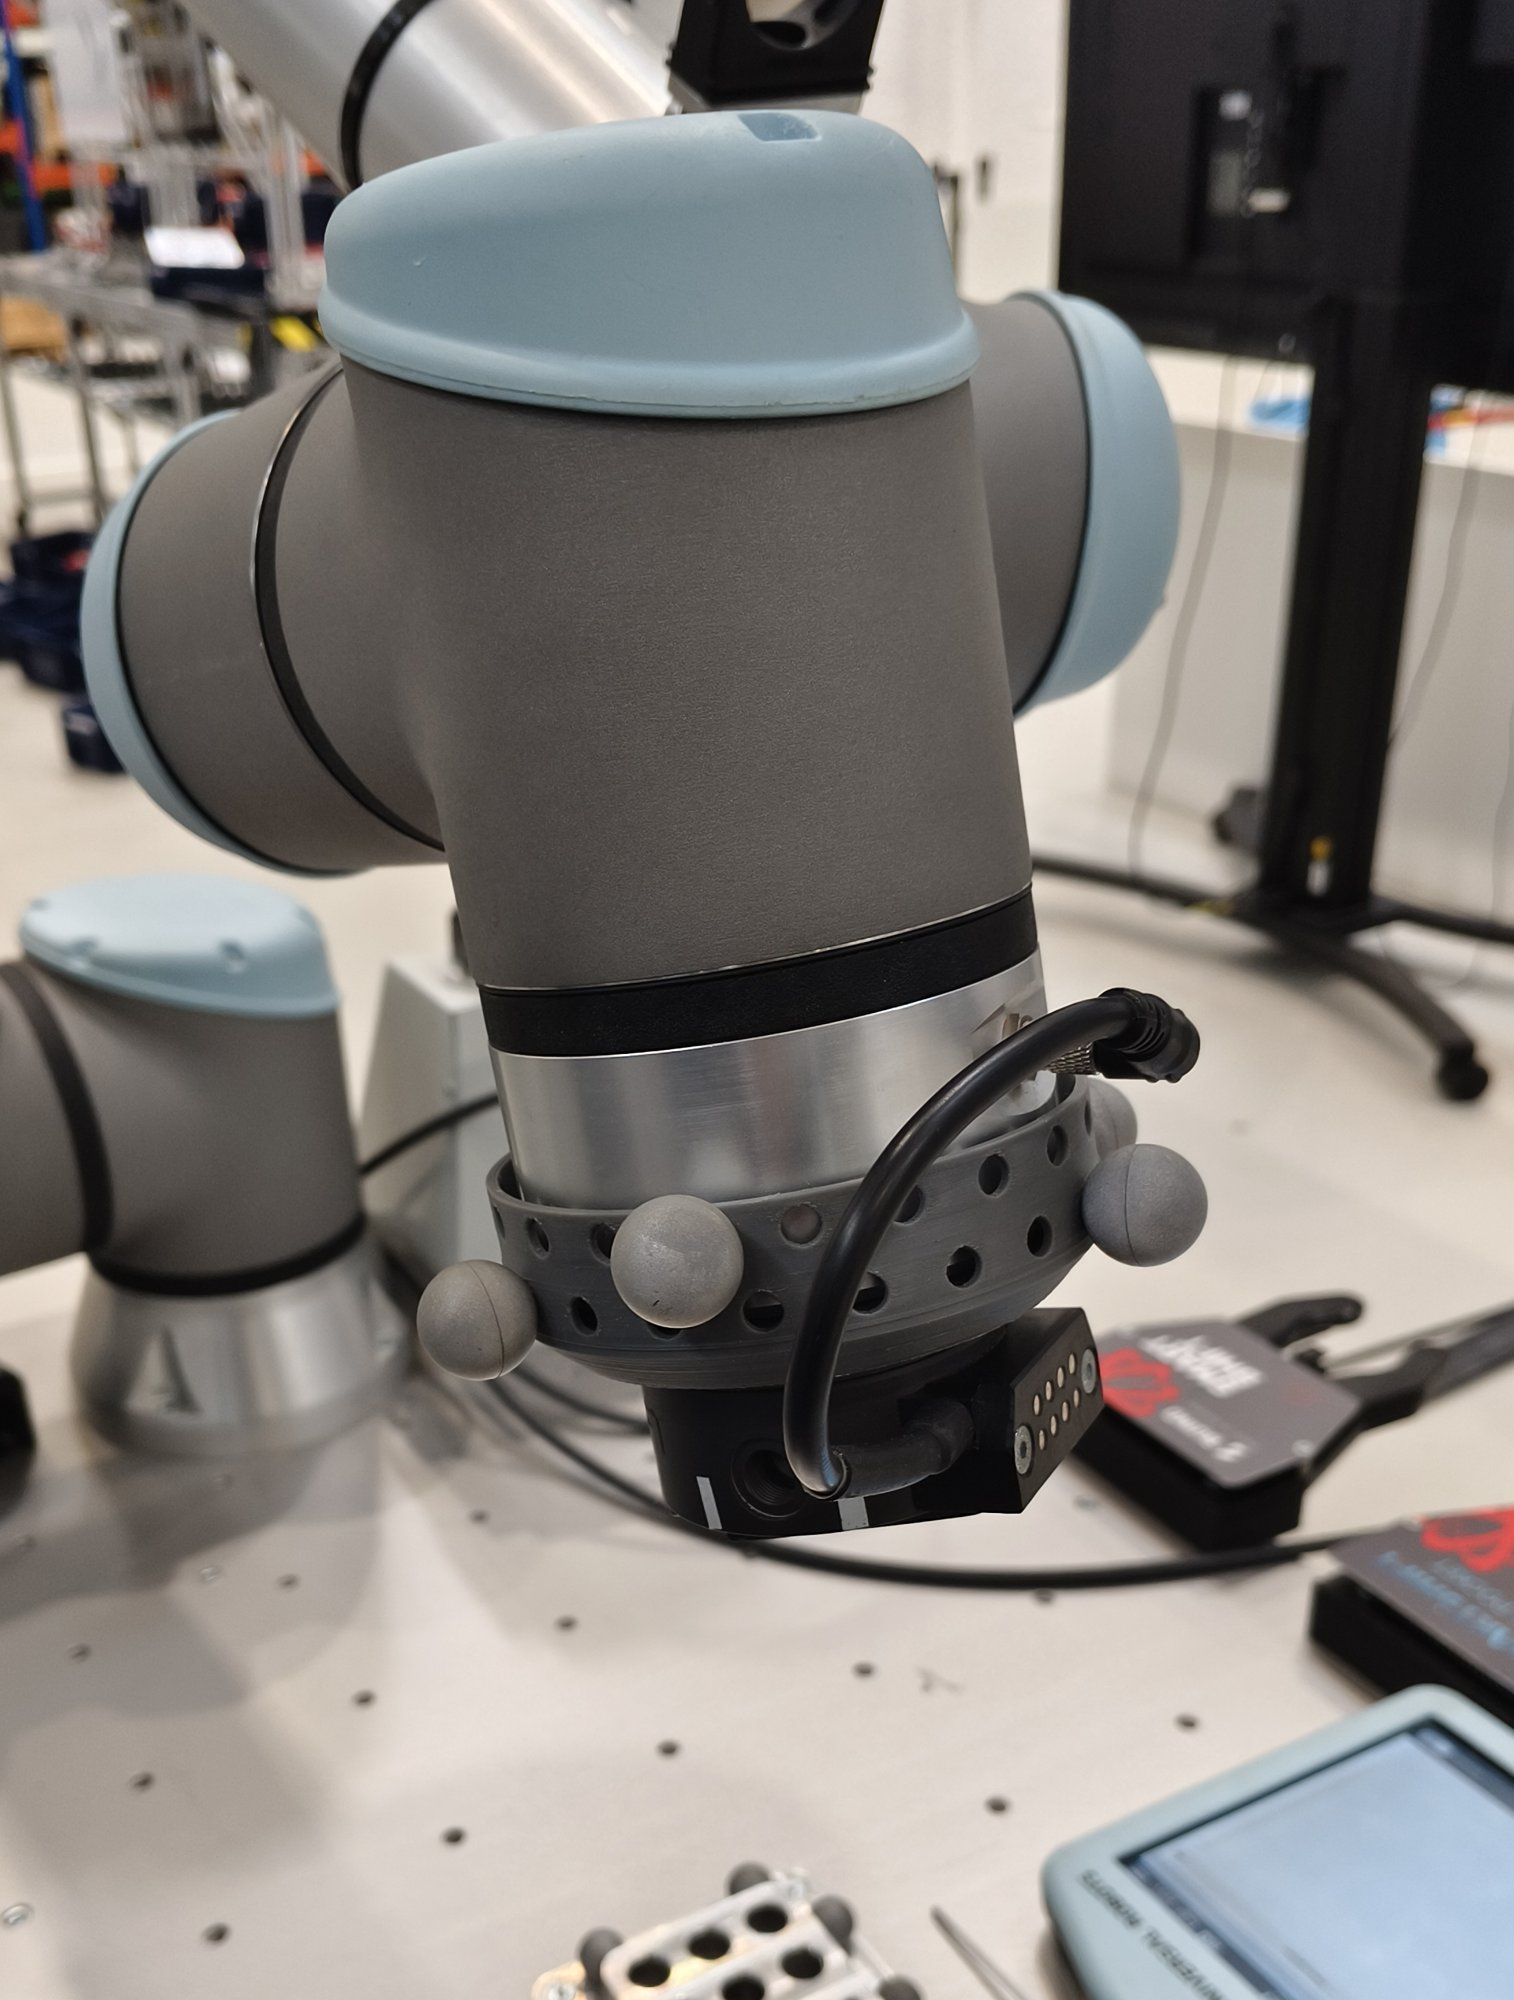
\includegraphics[height=5cm]{hero_tool_flange.jpg}
    \caption{Wrist~3 with the tool flange (\texttt{tool0}) and
      motion-capture markers.}
    \label{fig:collision-photo-flange}
  \end{subfigure}
  \caption{Platform bodies and arm attachments that enter the
    self-collision model.}
  \label{fig:collision-photos}
\end{figure}

The reduction to twelve pairs, listed in \cref{tab:collision-pairs},
removes pairs that are redundant rather than pairs that are harmless. An
attachment is dropped when the pair formed by its parent link and the
same platform body already keeps it clear. For the rings this holds with
any margin larger than their protrusion. For the tube holders it
required raising the minimum distance from \qty{0.08}{\meter} to
\qty{0.11}{\meter}, which leaves a clearance of about
\qty{5}{\centi\meter} for a dropped holder in its least favourable
orientation. The two largest holders sit on the forearm, the link that
most often dips towards the chassis during operation, and their pairs
with the chassis are kept explicitly. The dropped pairs are listed in a
comment of the task file but are not part of the model. Their effect on
solve time was not measured in isolation; the reduction cut the number
of distance queries per solve by \qty{62.5}{\percent}, and the UR safety
layer remains the last line of protection against a contact the reduced
set does not see.

\begin{table}[htbp]
  \centering
  \caption[Self-collision pairs before and after the reduction]{%
    Self-collision pairs between the arm and the two platform bodies,
    before (32) and after (12) the reduction. A dropped pair is covered
    by the pair of its parent link with the same platform body and the
    minimum distance of \qty{0.11}{\meter}.}
  \label{tab:collision-pairs}
  \begin{tabularx}{\linewidth}{@{}Xlcc@{}}
    \toprule
    Arm-side body & Protrusion & \texttt{hmi} & \texttt{chassis} \\
    \midrule
    \texttt{upper\_arm}, \texttt{forearm}, \texttt{wrist\_1}--\texttt{3}
      & link itself & kept (5) & kept (5) \\
    marker rings \texttt{ring2}, \texttt{ring2b}, \texttt{ring3}--\texttt{ring6}
      & $\le \qty{1}{\centi\meter}$ & dropped (6) & dropped (4) \\
    tube holders \texttt{bottom\_1}--\texttt{4}
      & \qtyrange{3}{6}{\centi\meter} & dropped (4) & dropped (4) \\
    tube holders \texttt{top\_3}, \texttt{top\_4} (forearm)
      & \qtyrange{3}{6}{\centi\meter} & dropped (2) & kept (2) \\
    \midrule
    Pairs before / after & & 17 / 5 & 15 / 7 \\
    \bottomrule
  \end{tabularx}
\end{table}

\Cref{fig:selfcollision-postures} shows two arm postures in which the
wrist comes close to the chassis. In both, the elbow is raised and the
forearm points downwards. In the first posture the three wrist links
arrive at the edge of the chassis top. In the second the forearm reaches
past that edge, and the wrist links lie beside the side wall of the
chassis, below the top plate. The pairs concerned are those of
\texttt{chassis} with \texttt{forearm\_link} and with
\texttt{wrist\_1\_link} to \texttt{wrist\_3\_link}.

\begin{figure}[htbp]
  \centering
  \begin{subfigure}[t]{0.544\textwidth}
    \centering
    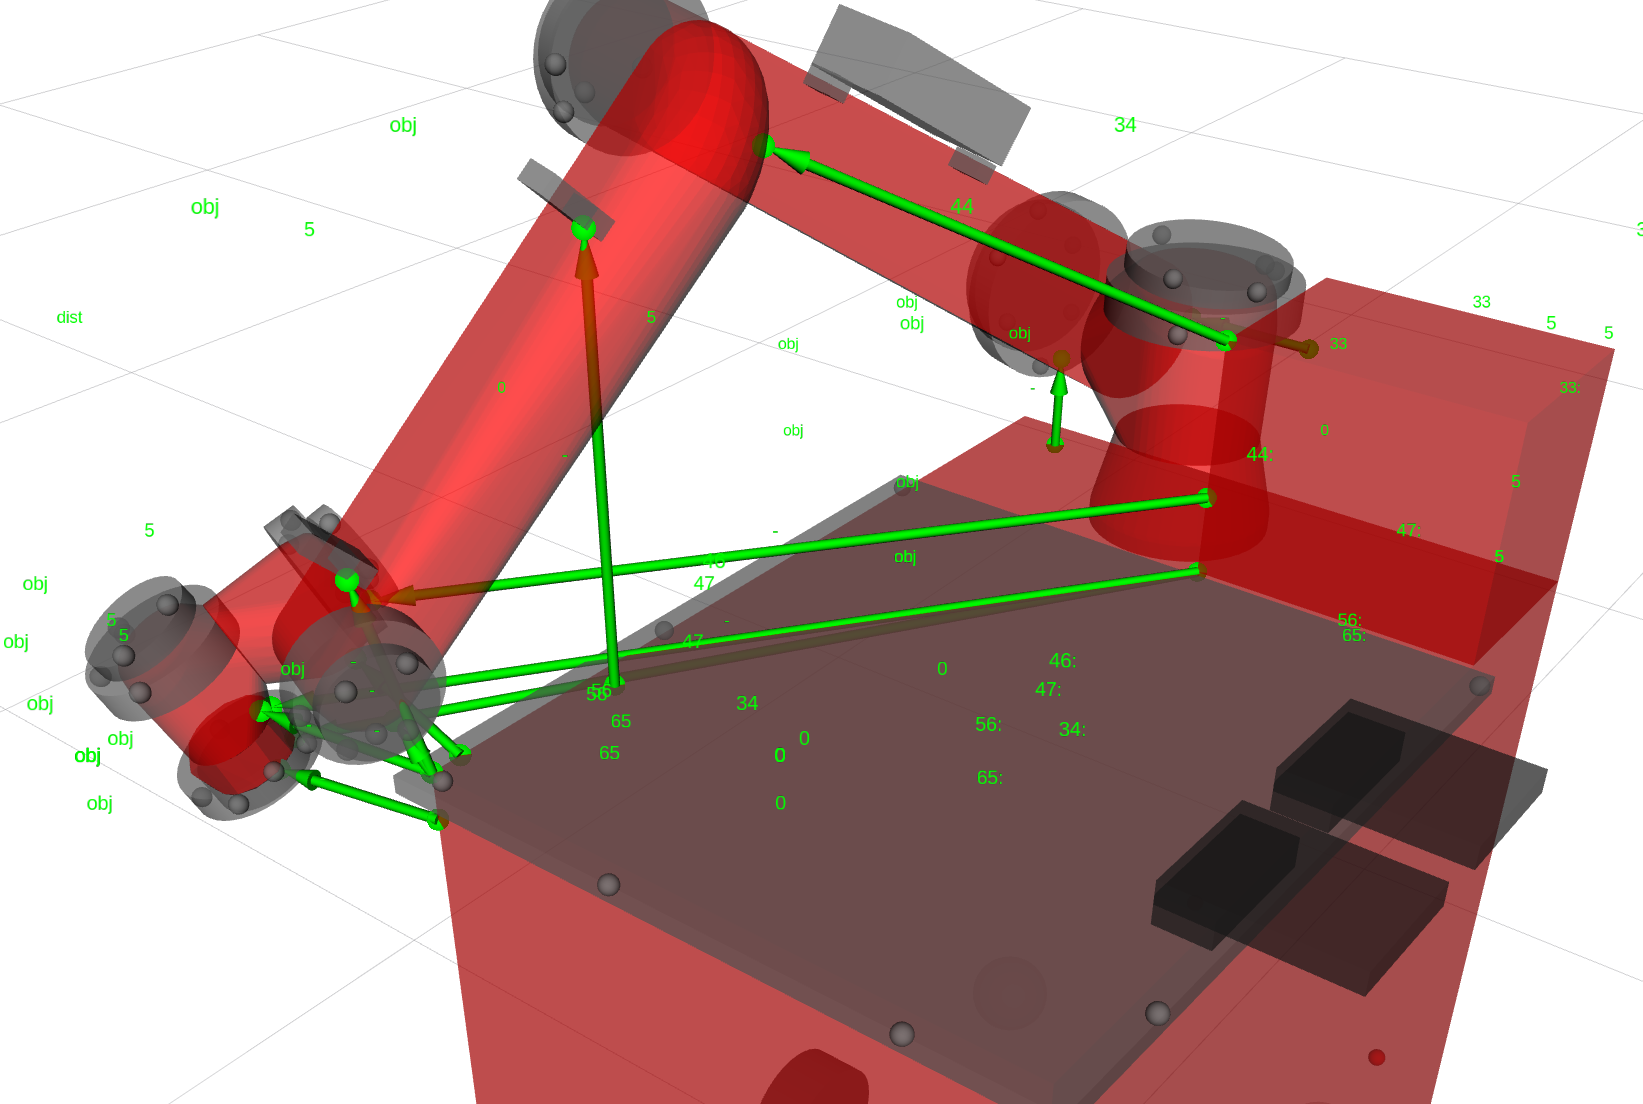
\includegraphics[width=\textwidth]{selfcollision_wrist_plate_edge.png}
    \caption{Wrist links at the edge of the chassis top}
    \label{fig:selfcollision-plate-edge}
  \end{subfigure}
  \hfill
  \begin{subfigure}[t]{0.436\textwidth}
    \centering
    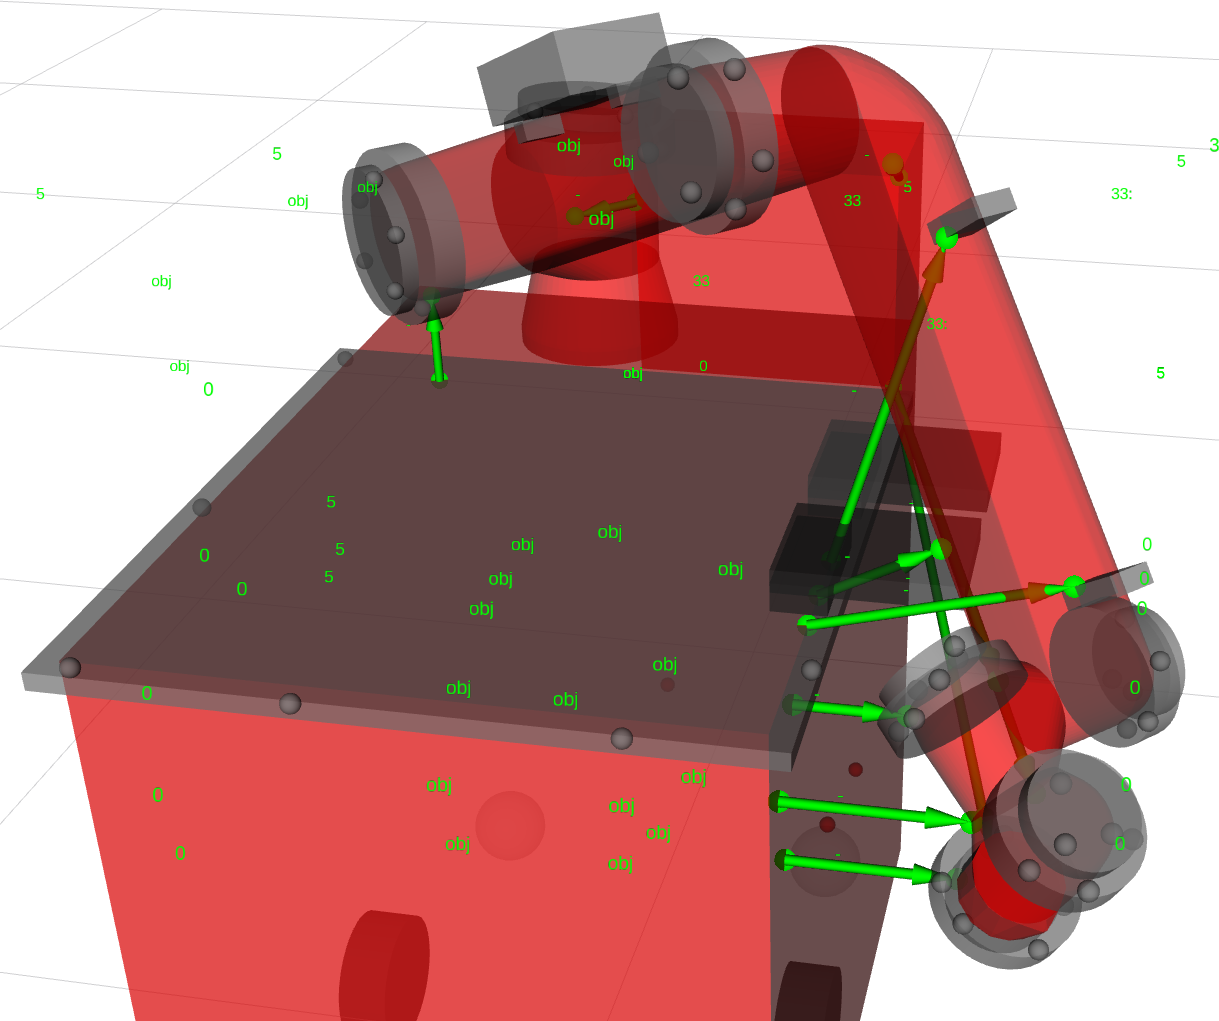
\includegraphics[width=\textwidth]{selfcollision_wrist_side_wall.png}
    \caption{Wrist links beside the side wall of the chassis}
    \label{fig:selfcollision-side-wall}
  \end{subfigure}
  \caption[Arm postures in which the wrist comes close to the chassis]{%
    Arm postures in which the wrist comes close to the chassis, drawn
    with the collision bodies of the model in RViz. Red bodies are the
    chassis, the operator panel (\texttt{hmi}) and the arm links; marker
    rings and tube holders are grey. Each green arrow joins the closest
    points of one body pair that the distance node evaluates. The green
    text is the label output of that node and is not evaluated here.}
  \label{fig:selfcollision-postures}
\end{figure}

The solver settings and the horizon are collected in
\cref{tab:mpc-config}. Three of them interact and are worth spelling
out. Only one SLQ iteration per solve is allowed. The solver starts a
new solve as soon as the previous one has finished
(\cref{sec:hw-interfaces}), so the previous solution, computed a few
hundred milliseconds earlier over a \qty{1.2}{\second} horizon, is a
usable initial guess; a second iteration would roughly double the solve
time and delay the next fresh observation by the same
amount~\cite{Farshidian2017SLQ}. The policy that the solver
publishes is declared valid for a \emph{solution time window} of
\qty{1.0}{\second}, shorter than the horizon; the bridge holds the robot
once a policy is exhausted rather than extrapolating it
(\cref{sec:hw-interfaces}). Real-time operation therefore requires

\begin{equation}
  2 \cdot \overline{t}_\mathrm{solve} \;<\; T_\mathrm{sol} \;<\; T ,
  \label{eq:rt-invariant}
\end{equation}

with $\overline{t}_\mathrm{solve}$ the average solve time,
$T_\mathrm{sol}$ the solution time window and $T$ the horizon: a policy
must arrive before the previous one expires, and it must not claim
validity beyond the horizon it was computed for. This invariant is
checked from the solver's diagnostics topic at the start of every
session and is the quantity that governs the failure mode analysed in
\cref{sec:hw-challenges}. \Cref{fig:rt-invariant} places the three
quantities on one time axis.

\begin{figure}[htbp]
  \centering
  \begin{tikzpicture}[
      font=\footnotesize,
      lbl/.style={font=\scriptsize, align=center},
      note/.style={font=\scriptsize, align=left},
      bar/.style={draw, minimum height=5.5mm, inner sep=0pt, anchor=west},
      tick/.style={thin, gray, dashed},
    ]
    % scale: 1 s = 6.5 cm
    \def\sT{7.8}    % horizon 1.2 s
    \def\sS{6.5}    % solution time window 1.0 s
    \def\sQ{3.0}    % 2 * average solve time, illustrative

    % --- guide lines --------------------------------------------------
    \draw[tick] (\sS,0.55) -- (\sS,-3.3);
    \draw[tick] (\sT,0.55) -- (\sT,-3.3);

    % --- bars ----------------------------------------------------------
    \node[bar, minimum width=\sT cm, fill=RWTHBlau100!12] (h) at (0,0) {};
    \node[lbl] at (\sT/2,0) {horizon $T = \qty{1.2}{\second}$};

    \node[bar, minimum width=\sS cm, fill=RWTHBlau100!25] (s) at (0,-1.0) {};
    \node[lbl] at (\sS/2,-1.0)
      {solution time window $T_\mathrm{sol} = \qty{1.0}{\second}$};

    \node[bar, minimum width=\sQ cm, fill=RWTHOrange100!30] (q) at (0,-2.0) {};
    \node[lbl] at (\sQ/2,-2.0) {$2\,\overline{t}_\mathrm{solve}$};

    % --- axis ----------------------------------------------------------
    \draw[-{Latex[length=1.8mm]}] (0,-3.0) -- (\sT+0.9,-3.0)
      node[right, font=\scriptsize] {$\tau$};
    \foreach \x/\t in {0/0} {
      \draw (\x,-2.9) -- (\x,-3.1) node[below, lbl] {\t};
    }
    \draw (\sS,-2.9) -- (\sS,-3.1) node[below, lbl] {$T_\mathrm{sol}$};
    \draw (\sT,-2.9) -- (\sT,-3.1) node[below, lbl] {$T$};

    % --- violation annotations ------------------------------------------
    \node[note, anchor=north west, text width=112mm] at (0,-3.55)
      {If $2\,\overline{t}_\mathrm{solve}$ reaches past $T_\mathrm{sol}$, a
       policy expires before its successor arrives and the bridge holds.
       If $T_\mathrm{sol}$ passed $T$, a policy would claim validity
       beyond the horizon it was computed for.};
  \end{tikzpicture}
  \caption[Real-time invariant of the \mpc{}--MRT loop]{%
    The three quantities of \cref{eq:rt-invariant} on one time axis, at
    the everyday operating point of \cref{tab:mpc-config}. The ordering
    $2\,\overline{t}_\mathrm{solve} < T_\mathrm{sol} < T$ is a design
    condition checked before a session, not a measurement, and the length
    of the $2\,\overline{t}_\mathrm{solve}$ bar is illustrative; the solve
    times actually reached on the two plants are reported in
    \cref{sec:hw-challenges}, where the \mpc{} loop runs at the wider
    Experiment~A setting.}
  \label{fig:rt-invariant}
\end{figure}

\begin{table}[!htbp]
  \centering
  \caption[\ocs{} operating point on \hero{}]{%
    \ocs{} operating point for on-robot operation, as configured in
    \texttt{task\_hardware.info}. Velocity limits appear twice by
    design: once as a soft constraint inside the optimisation and once
    as a hard clamp in the bridge.}
  \label{tab:mpc-config}
  \begin{tabularx}{\linewidth}{@{}lXl@{}}
    \toprule
    Group & Parameter & Value \\
    \midrule
    Model    & state / input dimension        & $9$ / $8$ \\
             & base frame, \ee{} frame        & \texttt{footprint}, \texttt{tool0} \\
             & fixed joints                   & both wheel joints \\
    \addlinespace
    Solver   & algorithm                      & SLQ \\
             & iterations per solve           & $1$ \\
             & threads                        & $8$ \\
             & backward-pass step, integrator & \qty{2}{\milli\second}, ODE45 \\
             & rollout step                   & \qty{10}{\milli\second} \\
             & feedback policy                & disabled (feed-forward) \\
    \addlinespace
    \mpc{}   & horizon $T$                    & \qty{1.2}{\second} \\
             & solution time window $T_\mathrm{sol}$ & \qty{1.0}{\second} \\
             & bridge loop rate $f_\mathrm{MRT}$ (\texttt{mrtDesiredFrequency}) & \qty{50}{\hz} \\
             & solve rate                     & $\min(f_\mathrm{MRT},\, 1/t_\mathrm{solve})$ \\
             & \texttt{mpcDesiredFrequency}   & \qty{10}{\hz}, warning threshold only \\
    \addlinespace
    Cost     & $R_\mathrm{base}$, $R_\mathrm{arm}$ & $0.085\,I_2$, $0.04\,I_6$ \\
             & $\mu_\mathrm{p}$, $\mu_\mathrm{o}$ (running and final) & $10$, $5$ \\
    \addlinespace
    Limits   & base velocity                  & \qty{\pm 0.1}{\meter\per\second}, \qty{\pm 0.1}{\radian\per\second} \\
             & arm joint velocity             & \qty{\pm 0.3}{\radian\per\second} \\
             & arm joint positions           & UR safety-panel limits \\
             & self-collision pairs, margin   & $12$, \qty{0.11}{\meter} \\
    \bottomrule
  \end{tabularx}
\end{table}

Derivatives are not written by hand. \ocs{} traces the cost terms, the
constraints and the system equation with CppAD and compiles the
resulting derivative code into shared libraries on first use, which is
the delay mentioned in
\cref{sec:distributed-arch}~\cite{CppAD,ocs2Toolbox}. The cache is keyed
by the model, not by the tuning: changing the kinematic model, the fixed
joints or the collision pair list invalidates it and requires a
regeneration, whereas changing a weight, a limit or the horizon takes
effect on the next restart. This distinction matters in practice,
because a stale cache silently keeps the old model while the
configuration file suggests otherwise.

% ---------------------------------------------------------------------
\section{Hardware Interfaces and ROS Control Layer Integration}
\label{sec:hw-interfaces}

The MRT bridge is the only component written specifically for this
deployment. It is the MRT client of the MPC--MRT split
(\cref{sec:sota-ocs2}) adapted to the real robot, and it closes the loop
between the \ocs{} policy and \texttt{ros2\_control} on the
IPC~\cite{ros2control}. Its practical role is to decouple the actuation
rate from the solve rate. A policy arrives only every few hundred
milliseconds, but it is a function of time over the solution time
window, so the bridge can evaluate it at the current time in every cycle
and keep commanding the robot between solves. The bridge is also the
place where a policy that has become too old is detected and replaced
by a hold.

The bridge has a single clock, the loop rate $f_\mathrm{MRT}$ set by
\texttt{mrtDesiredFrequency} in the task file. Each cycle publishes an
observation, collects a newly arrived policy, runs the checks of
\cref{tab:bridge-guards} and evaluates the policy into a base twist and
an arm setpoint. The observation also paces the solver: the \mpc{} node
solves inside the callback of each observation it receives, with a queue
depth of one and no throttle of its own~\cite{ocs2Toolbox}. The solve
rate on the robot is therefore $\min(f_\mathrm{MRT}, 1/t_\mathrm{solve})$,
with $t_\mathrm{solve}$ the duration of one solve. The
\texttt{mpcDesiredFrequency} entry of \qty{10}{\hz} does not throttle
anything on this path; the bridge uses it only as the warning threshold
in \cref{tab:bridge-guards}.

The loop rate was lowered from \qty{100}{\hz} to \qty{50}{\hz} after the
sessions reported in \cref{ch:hardware}, which ran at \qty{100}{\hz}.
At \qty{100}{\hz} the bridge sampled the base faster than its state
source changes: the drive controller publishes odometry at
\qty{50}{\hz}, so every second observation carried the same base pose
as the one before it. That doubled the observation traffic over the
network and the work of the bridge on the four-thread IPC without adding
information. The solver was not affected, because with solves of a few
hundred milliseconds it runs back to back at either rate. The lower rate
keeps the other requirements on the loop satisfied with margin. The base
twist is held for one cycle, which at the \qty{0.1}{\meter\per\second}
bound is a step of \qty{2}{\milli\meter} instead of
\qty{1}{\milli\meter}. The \qty{0.2}{\second} staleness window is still
checked ten times, and the \qty{0.5}{\second} command timeout of the
drive controller spans 25 cycles. The commanded arm speed is bounded by
the step clamp described below, independently of the loop rate. The
price is that a new policy may wait up to one cycle,
\qty{20}{\milli\second}, before it is first used.

Each cycle begins with an observation. The base pose $(p_x, p_y, \psi)$
is taken from the drive controller's odometry, with the yaw extracted
from the reported quaternion, and $\qarm$ is looked up by joint name in
\texttt{/joint\_states}; a missing joint aborts the cycle with a
throttled warning instead of silently inserting a zero. The observation
timestamp is the later of the two message stamps, expressed relative to
the origin fixed at the first accepted measurement, which is the
relative time axis that makes the deployment insensitive to clock
offsets.

Before the first command, the bridge performs a reset handshake with the
\mpc{} node. The initial reference must not move the robot, so the
bridge computes the current \ee{} pose by forward kinematics from the
latest observation and sends it as a two-knot target trajectory inside
the reset request: the solver starts by holding the pose the robot is
already in. The bridge guards the handshake against both ways it can
fail. It waits for
the reset service rather than assuming it exists, logs an actionable
error after \qty{15}{\second} and keeps waiting, and retries the request
if the response is lost---a single dropped reply over the network must
not leave the bridge dead. After a handshake the time-axis baseline is
reset as well, because the blocking call may have consumed several
seconds and the next observation would otherwise look like a time jump.
\Cref{fig:reset-handshake} shows the exchange and the two ways it can
fail.

\begin{figure}[htbp]
  \centering
  \begin{tikzpicture}[
      font=\footnotesize,
      head/.style={draw, rounded corners=1pt, align=center, inner sep=3.5pt,
                   minimum height=7mm, minimum width=36mm},
      life/.style={dashed, gray},
      msg/.style={-{Latex[length=2mm]}, thick},
      selfact/.style={draw, rounded corners=1pt, align=left, inner sep=3pt,
                      font=\scriptsize, fill=gray!10},
      lbl/.style={font=\scriptsize, align=center},
      note/.style={font=\scriptsize, align=left, text=RWTHOrange100},
    ]
    \node[head] (b) at (0,0)   {MRT bridge (IPC)};
    \node[head] (m) at (8.2,0) {\mpc{} node (external PC)};
    \draw[life] (b.south) -- (0,-7.3);
    \draw[life] (m.south) -- (8.2,-7.3);

    % --- 1: build the initial target --------------------------------
    \node[selfact, anchor=west] (a1) at (0.25,-1.15)
      {forward kinematics of the latest observation\\
       $\rightarrow$ two-knot target at the current \ee{} pose};

    % --- 2: probe the service ---------------------------------------
    \node[selfact, anchor=west] (a2) at (0.25,-2.5)
      {probe \texttt{\dots\_mpc\_reset}, one attempt per second};
    \node[note, anchor=east, align=right, text width=30mm] at (-0.3,-2.5)
      {after \qty{15}{\second}: actionable\\error, and keep waiting};

    % --- 3: request ---------------------------------------------------
    \draw[msg] (0,-3.7) -- (8.2,-3.7)
      node[lbl, midway, above] {reset request, target in the payload};

    % --- 4: solver resets --------------------------------------------
    \node[selfact, anchor=east] (a4) at (7.95,-4.6)
      {reset the solver; write the target\\into the reference manager};

    % --- 5: response ---------------------------------------------------
    \draw[msg] (8.2,-5.6) -- (0,-5.6)
      node[lbl, midway, above] {response};
    \node[note, anchor=east, align=right, text width=30mm] at (-0.3,-5.6)
      {response lost: hold and\\retry on the next cycle};

    % --- 6: baseline --------------------------------------------------
    \node[selfact, anchor=west] (a6) at (0.25,-6.6)
      {clear the time-axis baseline; handshake done};
  \end{tikzpicture}
  \caption[Reset handshake between the MRT bridge and the \mpc{} node]{%
    Reset handshake that precedes the first command. The bridge derives
    the initial reference from its own latest observation, so the solver
    starts by holding the pose the robot is already in. Both guards, in
    orange, sit in the bridge: it waits for the service rather than
    assuming it exists, and a lost response leaves it holding and
    retrying instead of dead. Clearing the time-axis baseline
    afterwards is necessary because the blocking call may have consumed
    several seconds, which the next observation would otherwise present as
    a time jump.}
  \label{fig:reset-handshake}
\end{figure}

The base command is the first two elements of the optimised input,
published as a stamped twist on \texttt{/cmd\_vel\_ocs2} rather than
directly on the drive controller's command topic. A \texttt{twist\_mux}
arbitrates between sources by priority, with manual teleoperation above
\ocs{}, so a higher-priority teleoperation source preempts or stops a
\qty{400}{\kilo\gram} platform that is executing an optimised
trajectory~\cite{twistMux}. The published twist is clamped to the same
base velocity bounds that the optimisation uses as a soft constraint; the
clamp is the hard backstop for the case where the soft constraint is
violated.

The arm command needs additional handling, because the joint-trajectory
controller accepts a position setpoint over its topic interface without
enforcing any velocity limit~\cite{ros2control}. The bridge samples the
optimised arm state \qty{0.6}{\second} ahead and publishes it as a single
trajectory point with that time from start, but it first clamps each
joint's step to
$\dot{q}_\mathrm{max} \cdot t_\mathrm{preview} = \qty{0.18}{\radian}$
around the currently measured position. Because the next cycle repeats
the computation \qty{20}{\milli\second} later, the arm still advances
towards the target, at a rate bounded by
\qty{0.3}{\radian\per\second}. When the clamp engages, the bridge warns;
frequent warnings indicate that the optimised state is jumping between
solves, which later proved useful as a diagnostic and is taken up in
\cref{sec:hw-challenges}.

Whenever the bridge cannot produce a trustworthy command it publishes a
hold: a zero twist and an arm trajectory pinned at the measured joint
positions. Getting this right required two details that are invisible in
the algorithm but decide whether the robot actually stops. The twist is
stamped at the moment of publication, because a hold issued right after
a blocking call would otherwise carry a stale stamp and be rejected by
the drive controller as timed out. The arm trajectory carries a zero
header stamp, which the controller reads as ``start now''; a wall-clock
stamp arrives a few milliseconds late and the whole trajectory is
rejected as ending in the past, so the hold never applies.
\Cref{tab:bridge-guards} lists the conditions that trigger a hold, and
\cref{fig:bridge-cycle} places them in the order the cycle evaluates
them.

\begin{figure}[htbp]
  \centering
  \begin{tikzpicture}[
      font=\footnotesize,
      act/.style={draw, rounded corners=1pt, align=center, inner sep=3.5pt,
                  minimum height=8mm, minimum width=56mm},
      guard/.style={act, fill=gray!10},
      hold/.style={act, draw=RWTHOrange100, thick, minimum width=22mm},
      cmd/.style={act, minimum width=40mm},
      flow/.style={-{Latex[length=2mm]}, thick},
      rail/.style={thick},
      lbl/.style={font=\scriptsize, align=center},
      side/.style={font=\scriptsize, align=left},
    ]
    % --- main column -------------------------------------------------
    \node[act]   (obs) at (0,0)
      {observation from odometry and \texttt{/joint\_states},\\
       stamped with the later of the two};
    \node[guard] (g1)  at (0,-1.6) {measurement age $> \qty{0.2}{\second}$?};
    \node[guard] (g2)  at (0,-2.9)
      {$\Delta t < 0$ or $\Delta t > \qty{0.5}{\second}$?};
    \node[guard] (g3)  at (0,-4.2) {reset handshake done?};
    \node[act]   (upd) at (0,-5.5)
      {publish the observation, fetch the latest policy\\
       (no policy received yet: end the cycle)};
    \node[guard] (g4)  at (0,-6.8) {no new policy for $2\,T_\mathrm{sol}$?};
    \node[guard] (g5)  at (0,-8.1) {remaining policy validity $\le 0$?};
    \node[act]   (ev)  at (0,-9.4)
      {evaluate the policy at \texttt{observation.time}\\
       $\rightarrow$ input $\uvec$, state $\svec$};
    \node[cmd]   (base) at (-2.6,-11.3)
      {clamp $v, \omega$ to $\pm 0.1$;\\
       stamp at publication\\
       $\rightarrow$ \texttt{twist\_mux}};
    \node[cmd]   (arm)  at (2.6,-11.3)
      {clamp the step to $\pm \qty{0.18}{\radian}$,\\
       then to the panel limits\\
       $\rightarrow$ joint-trajectory controller};

    % --- hold ---------------------------------------------------------
    \node[hold] (hd) at (6.2,-4.85) {hold};
    \node[side, anchor=north west, text width=21mm] at (5.15,-5.45)
      {no policy for $5\times$ the timeout: also re-arm the handshake};

    % --- main flow ----------------------------------------------------
    \draw[flow] (obs) -- (g1);
    \draw[flow] (g1)  -- (g2)  node[lbl, midway, left=1mm] {no};
    \draw[flow] (g2)  -- (g3)  node[lbl, midway, left=1mm] {no};
    \draw[flow] (g3)  -- (upd) node[lbl, midway, left=1mm] {yes};
    \draw[flow] (upd) -- (g4);
    \draw[flow] (g4)  -- (g5)  node[lbl, midway, left=1mm] {no};
    \draw[flow] (g5)  -- (ev)  node[lbl, midway, left=1mm] {no};
    \draw[flow] (0,-9.85) -- (0,-10.3) -| (base.north);
    \draw[flow] (0,-9.85) -- (0,-10.3) -| (arm.north);

    % --- guard exits to the hold rail ---------------------------------
    \draw[rail] (g1.east) -- (4.9,-1.6) node[lbl, pos=0.4, above] {yes};
    \draw[rail] (g4.east) -- (4.9,-6.8) node[lbl, pos=0.4, above] {yes};
    \draw[rail] (g5.east) -- (4.9,-8.1) node[lbl, pos=0.4, above] {yes};
    \draw[rail] (4.9,-1.6) -- (4.9,-8.1);
    \draw[flow] (4.9,-4.85) -- (hd.west);

    % --- left-hand exits ----------------------------------------------
    \draw[rail] (g2.west) -- (-4.6,-2.9) node[lbl, pos=0.35, above] {yes};
    \node[side, anchor=south east, text width=33mm] at (-4.6,-2.78)
      {drop the frame; after 20 in a row, re-baseline the time axis and
       re-handshake};
    \draw[rail] (g3.west) -- (-4.6,-4.2) node[lbl, pos=0.35, above] {no};
    \node[side, anchor=north east, text width=33mm] at (-4.6,-4.32)
      {run the handshake of \cref{fig:reset-handshake}; on success
       continue, on failure hold};
  \end{tikzpicture}
  \caption[One cycle of the MRT bridge]{%
    One cycle of the MRT bridge, which runs at \qty{50}{\hz} on the IPC.
    The guards are evaluated in the order shown; each either passes the
    cycle on or ends it in the hold, which publishes a zero twist stamped
    at publication together with an arm trajectory pinned at the measured
    positions under a zero header stamp. The arm step limit of
    \qty{0.18}{\radian} is the product of the arm velocity bound and the
    preview time, \qty{0.3}{\radian\per\second} $\times$
    \qty{0.6}{\second}, so the arm still advances towards the optimised
    state over successive cycles. Thresholds and their origin are listed
    in \cref{tab:bridge-guards}.}
  \label{fig:bridge-cycle}
\end{figure}

\begin{table}[htbp]
  \centering
  \caption[Guards implemented in the MRT bridge]{%
    Guards implemented in the MRT bridge. Most thresholds are launch
    arguments of the bridge; the policy timeout is derived from
    $T_\mathrm{sol}$, and the warning threshold from
    \texttt{mpcDesiredFrequency}, both in the task configuration file.}
  \label{tab:bridge-guards}
  \begin{tabularx}{\linewidth}{@{}lX@{}}
    \toprule
    Condition & Reaction \\
    \midrule
    Measurement older than \qty{0.2}{\second}
      & hold; the state estimate is not trusted \\
    Observation time steps backwards, or forwards by more than
    \qty{0.5}{\second}
      & drop the frame to protect the solver's time axis; after $20$
        consecutive drops, accept the new time as baseline and
        re-handshake \\
    Remaining policy validity below \qty{0.1}{\second}
      ($1/\texttt{mpcDesiredFrequency}$)
      & warn: the robot is outrunning the optimiser \\
    Policy validity exhausted
      & hold instead of evaluating a policy beyond its window \\
    No new policy for $2\,T_\mathrm{sol}$, at least \qty{1}{\second}
      & hold; the external PC or the link is assumed busy \\
    No new policy for $5\times$ that time, at least \qty{5}{\second}
      & re-run the reset handshake, on the assumption that the \mpc{}
        node restarted and no longer accepts the current observations \\
    Commanded arm step beyond the rate limit
      & clamp the step and warn \\
    \bottomrule
  \end{tabularx}
\end{table}

Below the bridge, the control chain is the production \hero{} stack with
two deliberate deviations. The UR driver is started in headless mode
with the joint-trajectory controller active, so that whole-body control
does not depend on an operator starting a program on the teach pendant;
the trade-off is that the pendant must be in remote mode when the driver
starts, otherwise the external control program has to be re-sent. The
controller stopper, which deactivates arm controllers when no
program runs on the arm, keeps both the joint-trajectory controller and
the drive controller in its list of controllers to leave alone. This
preserves the safety interlock of the arm while ensuring that a
protective stop does not silently drop the controller through which
\ocs{} actuates.

Two limitations of the integration follow from the choices above rather
than from tuning, and both bound what the experiments in the following
chapters can show. The controller's notion of where the robot is comes
from wheel odometry alone, so \ee{} poses reconstructed from the
internal state are consistent within a run but not absolute; and the
optimisation reasons about the robot's own geometry only, so a
whole-body plan is collision-free with respect to the platform and blind
to the workspace around it.
